\chapter{Developing SmartDoc: A Bias-Aware Clinical Simulation Platform}
\label{chap:ch4}

Building on the cognitive and empirical foundations discussed in
Chapters~\ref{chap:ch2} and~\ref{chap:ch3}, this chapter presents the
development of \textbf{SmartDoc}, a conversational clinical simulation platform
that enables medical students to practice diagnostic reasoning and recognize
cognitive bias in real time.

While virtual patients are established teaching tools, most focus on factual
knowledge or procedural competence rather than on the cognitive processes that
govern clinical decision-making. Bias-aware educational systems remain scarce
and typically rely on post-hoc analysis rather than interactive feedback.
SmartDoc addresses this gap through a hybrid design that integrates structured
dialogue control with large language models (LLMs) to support realistic
conversation, bias detection, and automated evaluation.

Fully neural, end-to-end approaches were rejected as they lack transparency and
educational control. Instead, SmartDoc combines rule-based pedagogical logic
with LLM dialogue generation, ensuring both realism and accountability.

This chapter describes the implementation of this architecture.
Section~\ref{sec:system_design} introduces the conceptual and pedagogical design.
Section~\ref{sec:tech_impl} outlines the technical implementation, including
algorithms, database architecture, and deployment.
Section~\ref{sec:mtb_workflow} illustrates a complete diagnostic workflow, and
Section~\ref{sec:ui} describes the user interfaces.
The chapter concludes with a summary~\ref{sec:summary} and a bridge to the empirical evaluation in
Chapter~\ref{chap:results}.

% ============================================================
\section{System Design}
\label{sec:system_design}

SmartDoc’s design draws on principles introduced in Chapter~\ref{chap:ch2},
including progressive disclosure, metacognitive scaffolding, and dual-process
reasoning. Its objective is to replicate authentic diagnostic interaction while
embedding cognitive safeguards.

\subsection{Pedagogical Foundations}

Three educational principles underpin SmartDoc:

\begin{enumerate}
  \item \textbf{Authenticity} — natural language interaction that mimics
  anamnesis, examination, and investigation ordering.
  \item \textbf{Bias Awareness} — real-time detection of reasoning patterns such
  as anchoring or premature closure, with prompts that encourage reflection
  without interrupting immersion.
  \item \textbf{Structured Reflection} — metacognitive checkpoints that prompt
  learners to articulate evidence, alternatives, and uncertainty.
\end{enumerate}

\subsection{Architectural Overview}

The platform follows a three-layer architecture:

\begin{itemize}
  \item \textbf{Domain logic} — pedagogical rules governing information
  disclosure and bias detection.
  \item \textbf{API layer} — communication, state management, and coordination
  between components.
  \item \textbf{Presentation layer} — browser-based interface for dialogue and
  feedback.
\end{itemize}

At its core, the \textbf{Intent-Driven Disclosure Manager} orchestrates three
processes:

\begin{enumerate}
  \item \textit{Intent classification} — mapping learner queries to structured
  diagnostic intents.
  \item \textit{Progressive disclosure} — revealing information incrementally as
  learners ask targeted questions.
  \item \textit{Bias monitoring} — detecting bias-prone behaviours and issuing
  reflective prompts.
\end{enumerate}

\begin{figure}[h]
\centering
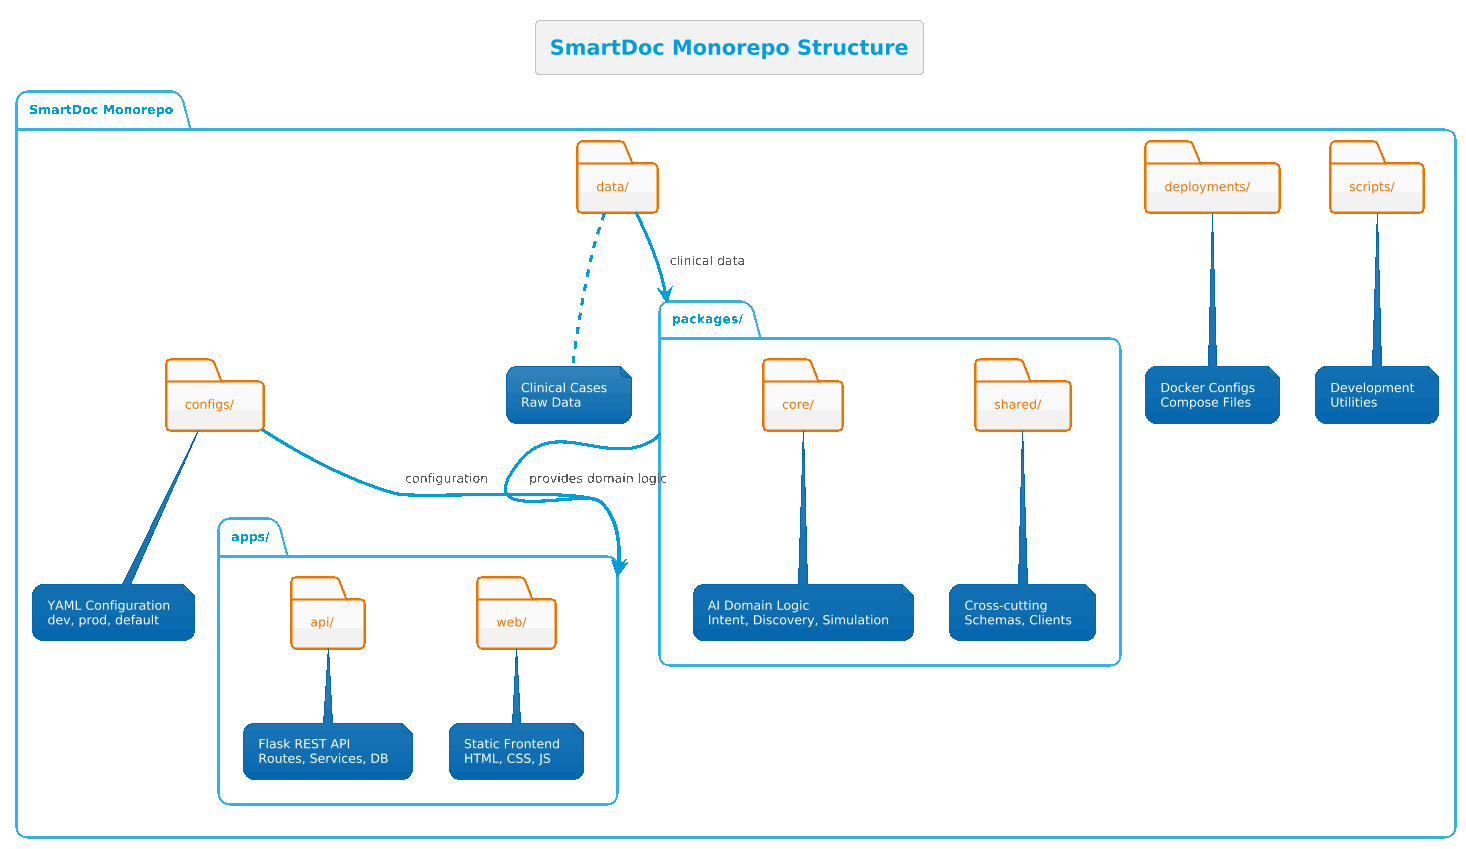
\includegraphics[width=0.70\textwidth]{figures/diagrams/high-level.png}
\caption{High-level architecture: three-layer design with modular components.}
\label{fig:high-level-arch}
\end{figure}

This modular architecture allows each component to be tested independently and
supports reproducibility across studies.

\subsection{Core Components}

SmartDoc integrates seven modules that together form a closed pedagogical loop.

\paragraph{Intent Classifier.}
Learner queries are mapped to a taxonomy of 33 diagnostic intents covering
anamnesis, examination, and investigations (Table~\ref{tab:intent_taxonomy}).
Context filtering ensures that queries are interpreted according to the current
diagnostic phase, supporting intuitive reasoning while maintaining structural
coherence.

\begin{table}[h]
\centering
\caption{Intent categories by diagnostic phase (selected examples).}
\label{tab:intent_taxonomy}
\setlength{\tabcolsep}{6pt}
\renewcommand{\arraystretch}{1.15}
\begin{tabular}{p{2.5cm} p{3.2cm} p{6.7cm} c}
\toprule
\textbf{Phase} & \textbf{Category} & \textbf{Example intents} & \textbf{Count} \\
\midrule
Anamnesis & Past Medical History &
\texttt{pmh\_general}, \texttt{pmh\_family\_history}, \texttt{pmh\_surgical\_history} & 3 \\
Anamnesis & History of Present Illness &
\texttt{hpi\_chief\_complaint}, \texttt{hpi\_onset\_duration}, \texttt{hpi\_fever}, \texttt{hpi\_chills} & 9 \\
Anamnesis & Medications &
\texttt{meds\_current}, \texttt{meds\_ra\_specific}, \texttt{meds\_full\_reconciliation} & 3 \\
Anamnesis & Social History &
\texttt{social\_smoking}, \texttt{social\_alcohol}, \texttt{social\_occupation} & 3 \\
Exam & General / System &
\texttt{exam\_vital}, \texttt{exam\_cardiovascular}, \texttt{exam\_respiratory} & 4 \\
Investigations & Laboratory &
\texttt{labs\_general}, \texttt{labs\_cbc}, \texttt{labs\_bnp} & 5 \\
Investigations & Imaging &
\texttt{imaging\_chest\_xray}, \texttt{imaging\_ct\_chest}, \texttt{imaging\_echo} & 6 \\
\bottomrule
\end{tabular}
\end{table}

\paragraph{Discovery Processor.}
Clinical facts are stored as modular \textit{information blocks} annotated by
level, prerequisites, and diagnostic importance. This mechanism enforces
progressive disclosure: information is revealed only when appropriate, promoting
active inquiry rather than passive information retrieval.

\paragraph{Bias Analyzer.}
Combining rule-based heuristics with LLM-assisted reasoning, the Bias Analyzer
monitors for anchoring, confirmation, and premature closure. When bias patterns
emerge, the system issues non-intrusive prompts such as:
\emph{“What else could explain these findings?”}

\paragraph{Clinical Evaluator.}
A single-LLM evaluator scores learner performance across three dimensions:
information gathering, diagnostic accuracy, and cognitive bias awareness.
Structured rubrics and strict temperature control ensure consistency between
evaluations.

\paragraph{Simulation Engine and Responders.}
The Simulation Engine manages the learning loop—query, classification,
disclosure, bias analysis, and response generation. Responder modules produce
context-appropriate replies: conversational for anamnesis, objective for
examinations, and concise for laboratory or imaging results.

\paragraph{Session Management.}
All interactions are logged with timestamps, generating comprehensive reasoning
traces used for feedback, assessment, and research.

\subsection{Case Modelling and Bias Integration}

Each SmartDoc case embeds pedagogical logic directly in its structure, linking
bias triggers, learning objectives, and reflection prompts.

\paragraph{Information blocks.}
Every block defines its level of inquiry, prerequisites, criticality, and
trigger intents. This schema supports both shallow and deep questioning, mirroring
expert diagnostic reasoning.

\paragraph{Bias triggers.}
Metadata identify potential anchors (e.g., misleading imaging findings),
contradictory evidence, and corrective prompts. When a learner focuses
excessively on one hypothesis despite conflicting data, a bias card is displayed
inviting reconsideration.

\paragraph{Educational scaffolding.}
Repeated unproductive queries activate dynamic hints, e.g.,
\emph{“Maybe you could check her previous hospital records?”}
This adaptive feedback maintains learner engagement while avoiding frustration.

\paragraph{Reflection prompts.}
At case closure, learners answer structured metacognitive questions on evidence,
counter-evidence, and alternatives. These responses foster deliberate reflection
(System~2 reasoning) and make clinical judgement processes explicit.

\paragraph{Prototype case.}
The pilot case adapts Mull~et~al.~\cite{mull_cognitive_2015}, where an elderly
woman with dyspnoea was misdiagnosed with heart failure due to anchoring bias.
SmartDoc reproduces this scenario through controlled framing, contradictory
findings, and a critical discovery—immunosuppressant therapy with infliximab.

% ============================================================
\section{Technical Implementation}
\label{sec:tech_impl}

\subsection{Technology Stack}

SmartDoc is built on a modular, containerised architecture designed for
reproducibility and portability across research and educational settings.

\begin{table}[h]
\centering
\caption{Core technologies and versions.}
\label{tab:core_stack}
\setlength{\tabcolsep}{6pt}
\renewcommand{\arraystretch}{1.12}
\begin{tabular}{p{3.2cm} p{4.0cm} p{2.0cm}}
\toprule
\textbf{Component} & \textbf{Technology} & \textbf{Version} \\
\midrule
Backend Framework & Flask & 3.0+ \\
Language & Python & 3.13+ \\
Dependency Mgmt & Poetry & 1.8+ \\
ORM \& Migrations & SQLAlchemy + Alembic & 2.0+ \\
Data Validation & Pydantic & 2.0+ \\
LLM Interface & Ollama & Latest \\
LLM Model & Gemma 3:4b-it-q4\_K\_M & 4B params \\
Frontend & HTML/CSS/JS & ES2020+ \\
Containerisation & Docker + Compose & 24.0+ \\
Prod Server & Gunicorn & 21.0+ \\
\bottomrule
\end{tabular}
\end{table}

\subsection{Execution Pipeline}

SmartDoc's processing loop mirrors a diagnostic encounter:

\begin{enumerate}
  \item Learner submits a query.
  \item Intent classified through hybrid LLM–rules pipeline.
  \item Discovery Processor reveals relevant information blocks.
  \item Phase-appropriate responder generates system reply.
  \item Bias Analyzer evaluates reasoning patterns.
  \item Events are logged and session state updated.
\end{enumerate}

Ambiguous queries trigger clarification requests rather than errors, preserving
conversation flow and cognitive authenticity.

\subsection{Intent-Driven Progressive Disclosure}
\label{sec:algo_progressive}

\noindent
The following pseudocode illustrates how the system governs information revelation,
educational scaffolding, and bias monitoring during each learner interaction.

\begin{verbatim}
Input: user_query, session_context, revealed_blocks
Output: information_blocks, educational_hints, bias_warnings

1:  phase ← session_context.current_phase
2:  available ← filter_intents_by_phase(phase)
3:  cls ← LLM_classify(user_query, available)
4:  if cls.confidence < 0.30 then
5:      return request_clarification(user_query, available)
6:  end if
7:  intent ← cls.intent_id
8:  mapped ← get_intent_block_mappings(intent, case)
9:  eligible ← filter_by_prerequisites(mapped, revealed_blocks)

10: // Just-in-time scaffolding
11: if intent == "meds_ra_specific_initial_query" then
12:     n ← count_previous_queries(intent, session)
13:     if n > 1 AND not revealed("critical_infliximab") then
14:         hint ← "Maybe you could check her previous hospital records?"
15:         return (eligible, hint, None)
16:     end if
17: end if

18: // Real-time bias check
19: focus ← calculate_focus(session_context.working_diagnosis)
20: if focus > 0.70 then
21:     contra ← detect_contradictions(revealed_blocks, session_context.working_diagnosis)
22:     if not empty(contra) then
23:         warn ← make_bias_warning("anchoring",
             "What else could explain these findings?")
24:         return (eligible, None, warn)
25:     end if
26: end if

27: return (eligible, None, None)
\end{verbatim}

\noindent
This algorithm operationalises progressive disclosure and scaffolding, ensuring
learners earn critical information through inquiry rather than direct
presentation.

\newpage

\subsection{Bias Detection and Warning System}
\label{sec:algo_bias}

\noindent
The following pseudocode illustrates how the system continuously evaluates reasoning
focus and evidence weighting to detect cognitive bias.

\begin{verbatim}
Input: session_history, current_hypothesis, revealed_information
Output: bias_warning or None

1:  recent ← last_n(session_history.queries, 5)
2:  f_ratio ← focus_ratio(recent, current_hypothesis)

3:  // Anchoring bias
4:  if f_ratio > 0.70 then
5:      contra ← detect_contradictions(revealed_information, current_hypothesis)
6:      if not empty(contra) then
7:          log_bias("anchoring", evidence=contra)
8:          return warn("anchoring",
              "You seem focused on one diagnosis.
              What else could explain this?",
              "moderate")
9:      end if
10: end if

11: // Confirmation bias
12: s ← count_supporting(recent, current_hypothesis)
13: r ← count_refuting(recent, current_hypothesis)
14: if s > 0 and r == 0 and len(recent) >= 4 then
15:     log_bias("confirmation", pattern="seeking only supporting evidence")
16:     return warn("confirmation",
                   "Consider evidence that might contradict your hypothesis",
                   "low")
17: end if

18: // Premature closure
19: needed ← critical_blocks(case)
20: have ← intersect(needed, revealed_information)
21: if len(have) < 0.6 * len(needed) and diagnosis_submitted(session_history) then
22:     log_bias("premature_closure", coverage=len(have))
23:     return warn("premature_closure", None, "high")
24: end if

25: return None
\end{verbatim}

\begin{figure}[h]
\centering
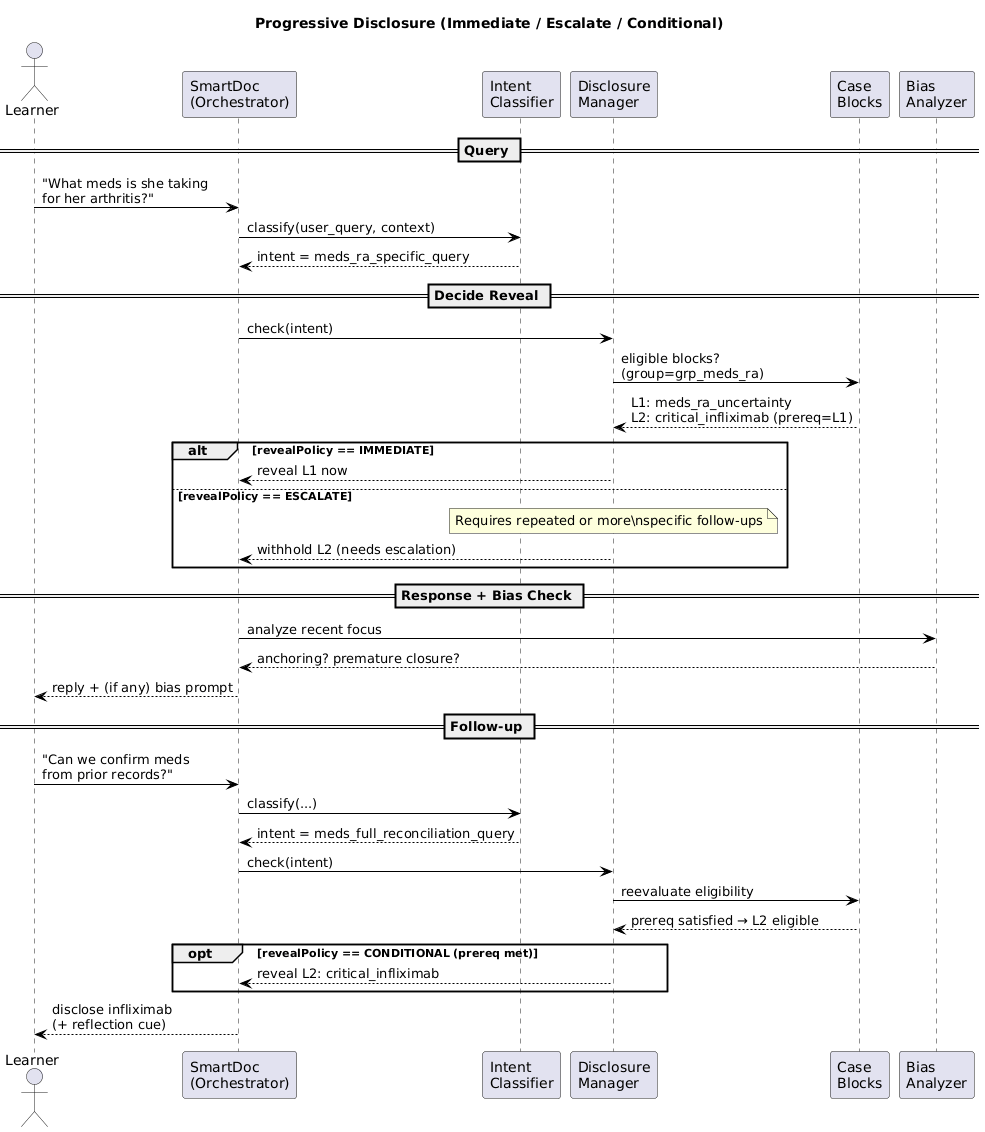
\includegraphics[width=0.70\textwidth]{figures/diagrams/progressive-disclosure.png}
\caption{Progressive disclosure sequence: from query to information revelation with prerequisite checking.}
\label{fig:progressive-disclosure}
\end{figure}

These rules convert cognitive-bias theory into actionable, real-time feedback.

\subsection{Classification Refinements and Accuracy}

Iterative testing revealed two critical issues that were addressed through
systematic refinement. First, queries about past medical history were
misclassified as medication requests due to insufficient negative examples.
Enhanced intent definitions with explicit negative constraints improved
accuracy from 57\% to >95\%. Second, cross-phase acceptance errors (e.g.,
medication queries during examination) were eliminated through strict phase
gating. These refinements demonstrate the evolution from prototype to
production-ready system (Table~\ref{tab:intent_accuracy}).

\begin{table}[h]
\centering
\caption{Intent classification accuracy improvements through iterative refinement.}
\label{tab:intent_accuracy}
\setlength{\tabcolsep}{6pt}
\renewcommand{\arraystretch}{1.15}
\begin{tabular}{lccc}
\toprule
\textbf{Configuration} & \textbf{PMH vs.\ Meds} & \textbf{Cross-phase errors} & \textbf{Overall} \\
\midrule
Baseline (generic defs.) & 57\% & 23\% & 78\% \\
+ Enhanced definitions & 95\% & 18\% & 87\% \\
+ Strict context filtering & 95\% & 0\% & 96\% \\
\bottomrule
\end{tabular}
\end{table}

\subsection{LLM Integration and Validation}

SmartDoc operates with a local \textbf{Ollama} host using the quantised
\texttt{gemma3:4b-it-q4\_K\_M} model for intent classification, dialogue, and
evaluation. This configuration balances privacy, performance, and accuracy
($>95$\% valid JSON outputs). Module-specific temperature settings balance
determinism and naturalness (Table~\ref{tab:temps}). Pydantic schema validation
guarantees reliable structured outputs; when validation fails, fallback
mechanisms ensure uninterrupted learning flow.

\begin{table}[h]
\centering
\caption{LLM temperature settings by module.}
\label{tab:temps}
\setlength{\tabcolsep}{8pt}
\renewcommand{\arraystretch}{1.12}
\begin{tabular}{l c p{7cm}}
\toprule
\textbf{Module} & \textbf{Temp.} & \textbf{Rationale} \\
\midrule
Intent Classification & 0.2 & High consistency; minimal variability \\
Clinical Evaluation & 0.3 & Reproducible scoring; fairness across sessions \\
Responders (dialogue) & 0.5 & Natural family dialogue with limited variability \\
Responders (labs) & 0.3 & Deterministic, professional reporting \\
\bottomrule
\end{tabular}
\end{table}

\subsection{Data Architecture}

Persistent data are stored in an SQLite database with an event-driven
architecture.
Entities include \textit{sessions, messages, discoveries, bias\_events,}
and \textit{evaluations.}
In-memory state ensures real-time performance, while automatic logging
maintains complete reasoning traces.

\begin{figure}[h]
\centering
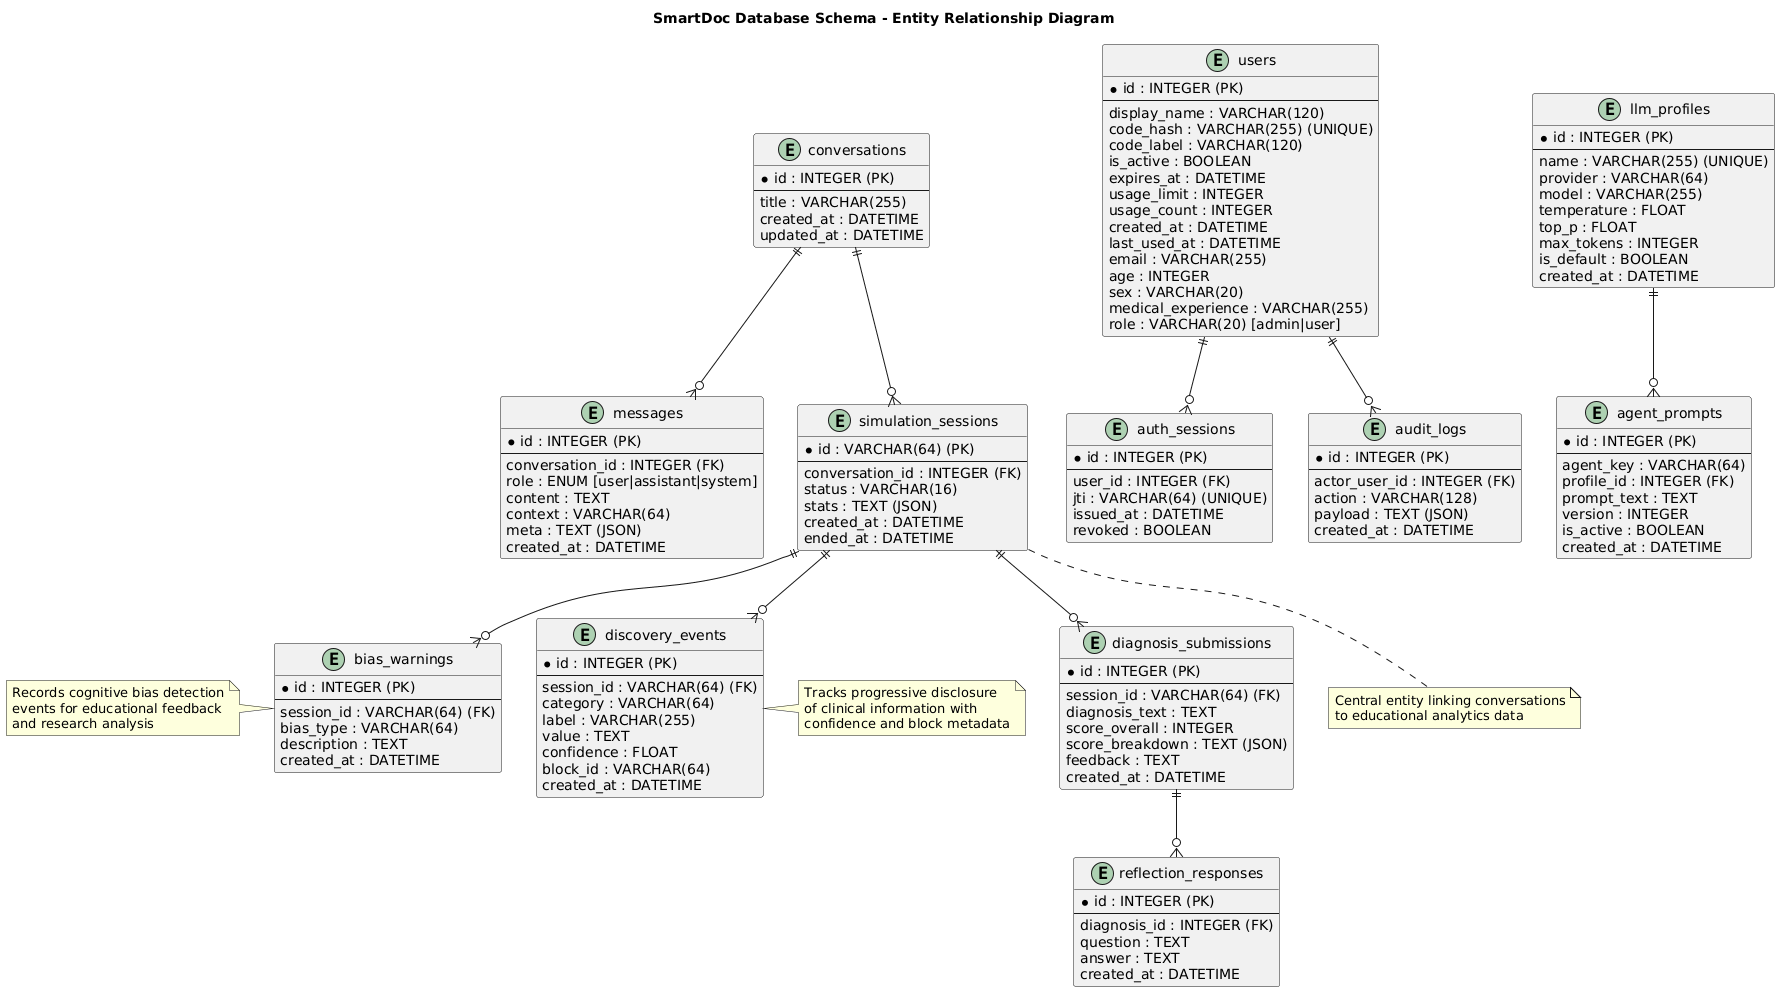
\includegraphics[width=0.82\textwidth]{figures/diagrams/erdb.png}
\caption{Conceptual schema: capturing reasoning traces, bias events, and reflection data.}
\label{fig:db_schema}
\end{figure}

\subsection{Deployment and Scalability}

SmartDoc runs as a containerised application with three services:
\textit{Flask API}, \textit{Ollama LLM Host}, and \textit{SQLite Database}.
Docker ensures reproducibility across machines and institutions.
Two deployment modes are supported:
(i)~local for research and privacy, and
(ii)~cloud for larger cohorts.
Structured logs capture latency and fallback events for monitoring.

% ============================================================
\section{Example Workflow: The Miliary Tuberculosis Case}
\label{sec:mtb_workflow}

This section demonstrates SmartDoc in practice through a full diagnostic
workflow (Session~\texttt{SESS\_0W451OZEJ}).
The case is based on Mull~et~al.~\cite{mull_cognitive_2015}, where an elderly
Spanish-speaking woman with dyspnoea was repeatedly misdiagnosed with heart
failure.

\subsection{Case Overview}

\noindent\textbf{Presentation:} 85-year-old Spanish-speaking woman with
progressive dyspnoea.
\textbf{Framing:} history of ``heart failure''.
\textbf{Correct diagnosis:} miliary tuberculosis related to infliximab therapy.
\textbf{Common misdiagnosis:} acute heart failure exacerbation.

\subsection{Phase Highlights}

\textbf{Anamnesis.} The learner identifies comorbidities (diabetes,
hypertension, rheumatoid arthritis).
After repeated queries about RA medication, the scaffolding hint—``check previous hospital records''—leads to discovery of infliximab use (critical finding).

\textbf{Examination.} Normal heart sounds and absence of oedema contradict the
initial hypothesis of heart failure.
Diffuse crackles are observed, remaining ambiguous until imaging.

\textbf{Investigations.} The chest X-ray suggests ``pulmonary vascular
congestion'', triggering an anchoring warning.
Subsequent CT reveals miliary nodules, and the echocardiogram confirms a normal
ejection fraction, prompting diagnostic revision.

\begin{table}[h]
\centering
\caption{Information revealed by category and timing (Session~\texttt{SESS\_0W451OZEJ}).}
\label{tab:discoveries_mtb}
\begin{tabular}{lccc}
\toprule
\textbf{Category} & \textbf{Count} & \textbf{Critical Findings} & \textbf{Timeline} \\
\midrule
Presenting symptoms & 6 & None & First 2 min \\
Current medications & 3 & Infliximab & min~\(\sim\)7 \\
Physical examination & 3 & None & 7--10 min \\
Imaging & 3 & Miliary nodules; normal echo & 10--15 min \\
Diagnostic results & 3 & None & 15--18 min \\
\midrule
\textbf{Total} & \textbf{18} & \textbf{2 critical} & \textbf{18 min} \\
\bottomrule
\end{tabular}
\end{table}

\subsection{Outcome and Reflection}

The learner submits \emph{miliary tuberculosis} as the final diagnosis
(Information~75, Accuracy~88, Bias~80 → Overall 81/100).
Reflection responses demonstrate awareness of contradictory evidence and
alternative hypotheses, confirming engagement of analytic reasoning.

\paragraph{Educational impact.}
This session demonstrates SmartDoc's pedagogical mechanisms in practice.
Progressive disclosure required 17 targeted queries to reveal 18 information
blocks, evidencing active inquiry rather than passive reading.
The just-in-time hint successfully guided medication reconciliation after two
unsuccessful attempts.
Bias detection triggered appropriately when preliminary imaging suggested heart
failure, logged as an anchoring warning.
Structured reflection showed explicit evidence integration (infliximab
$\rightarrow$ TB risk), acknowledgement of contradictions (normal echo vs.\
elevated BNP), and systematic consideration of alternatives.
Intent classification achieved 100\% accuracy (17/17 correct), while median
response latency remained under 6~seconds per turn—confirming that the system
met both technical and pedagogical objectives in this authentic diagnostic
scenario.

\newpage
% ============================================================
\section{User Interfaces}
\label{sec:ui}

SmartDoc’s user interfaces translate technical architecture into accessible,
low-friction learning tools.

\subsection{Simulation Interface}

The simulation is a single-page web application divided into four tabs:
\textit{Patient Information, Clinical Interview, Physical Examination,} and
\textit{Labs \& Imaging.}
Interactions occur via chat-based dialogue that distinguishes student (blue) and
system (gray) messages.

\begin{figure}[h]
  \centering
  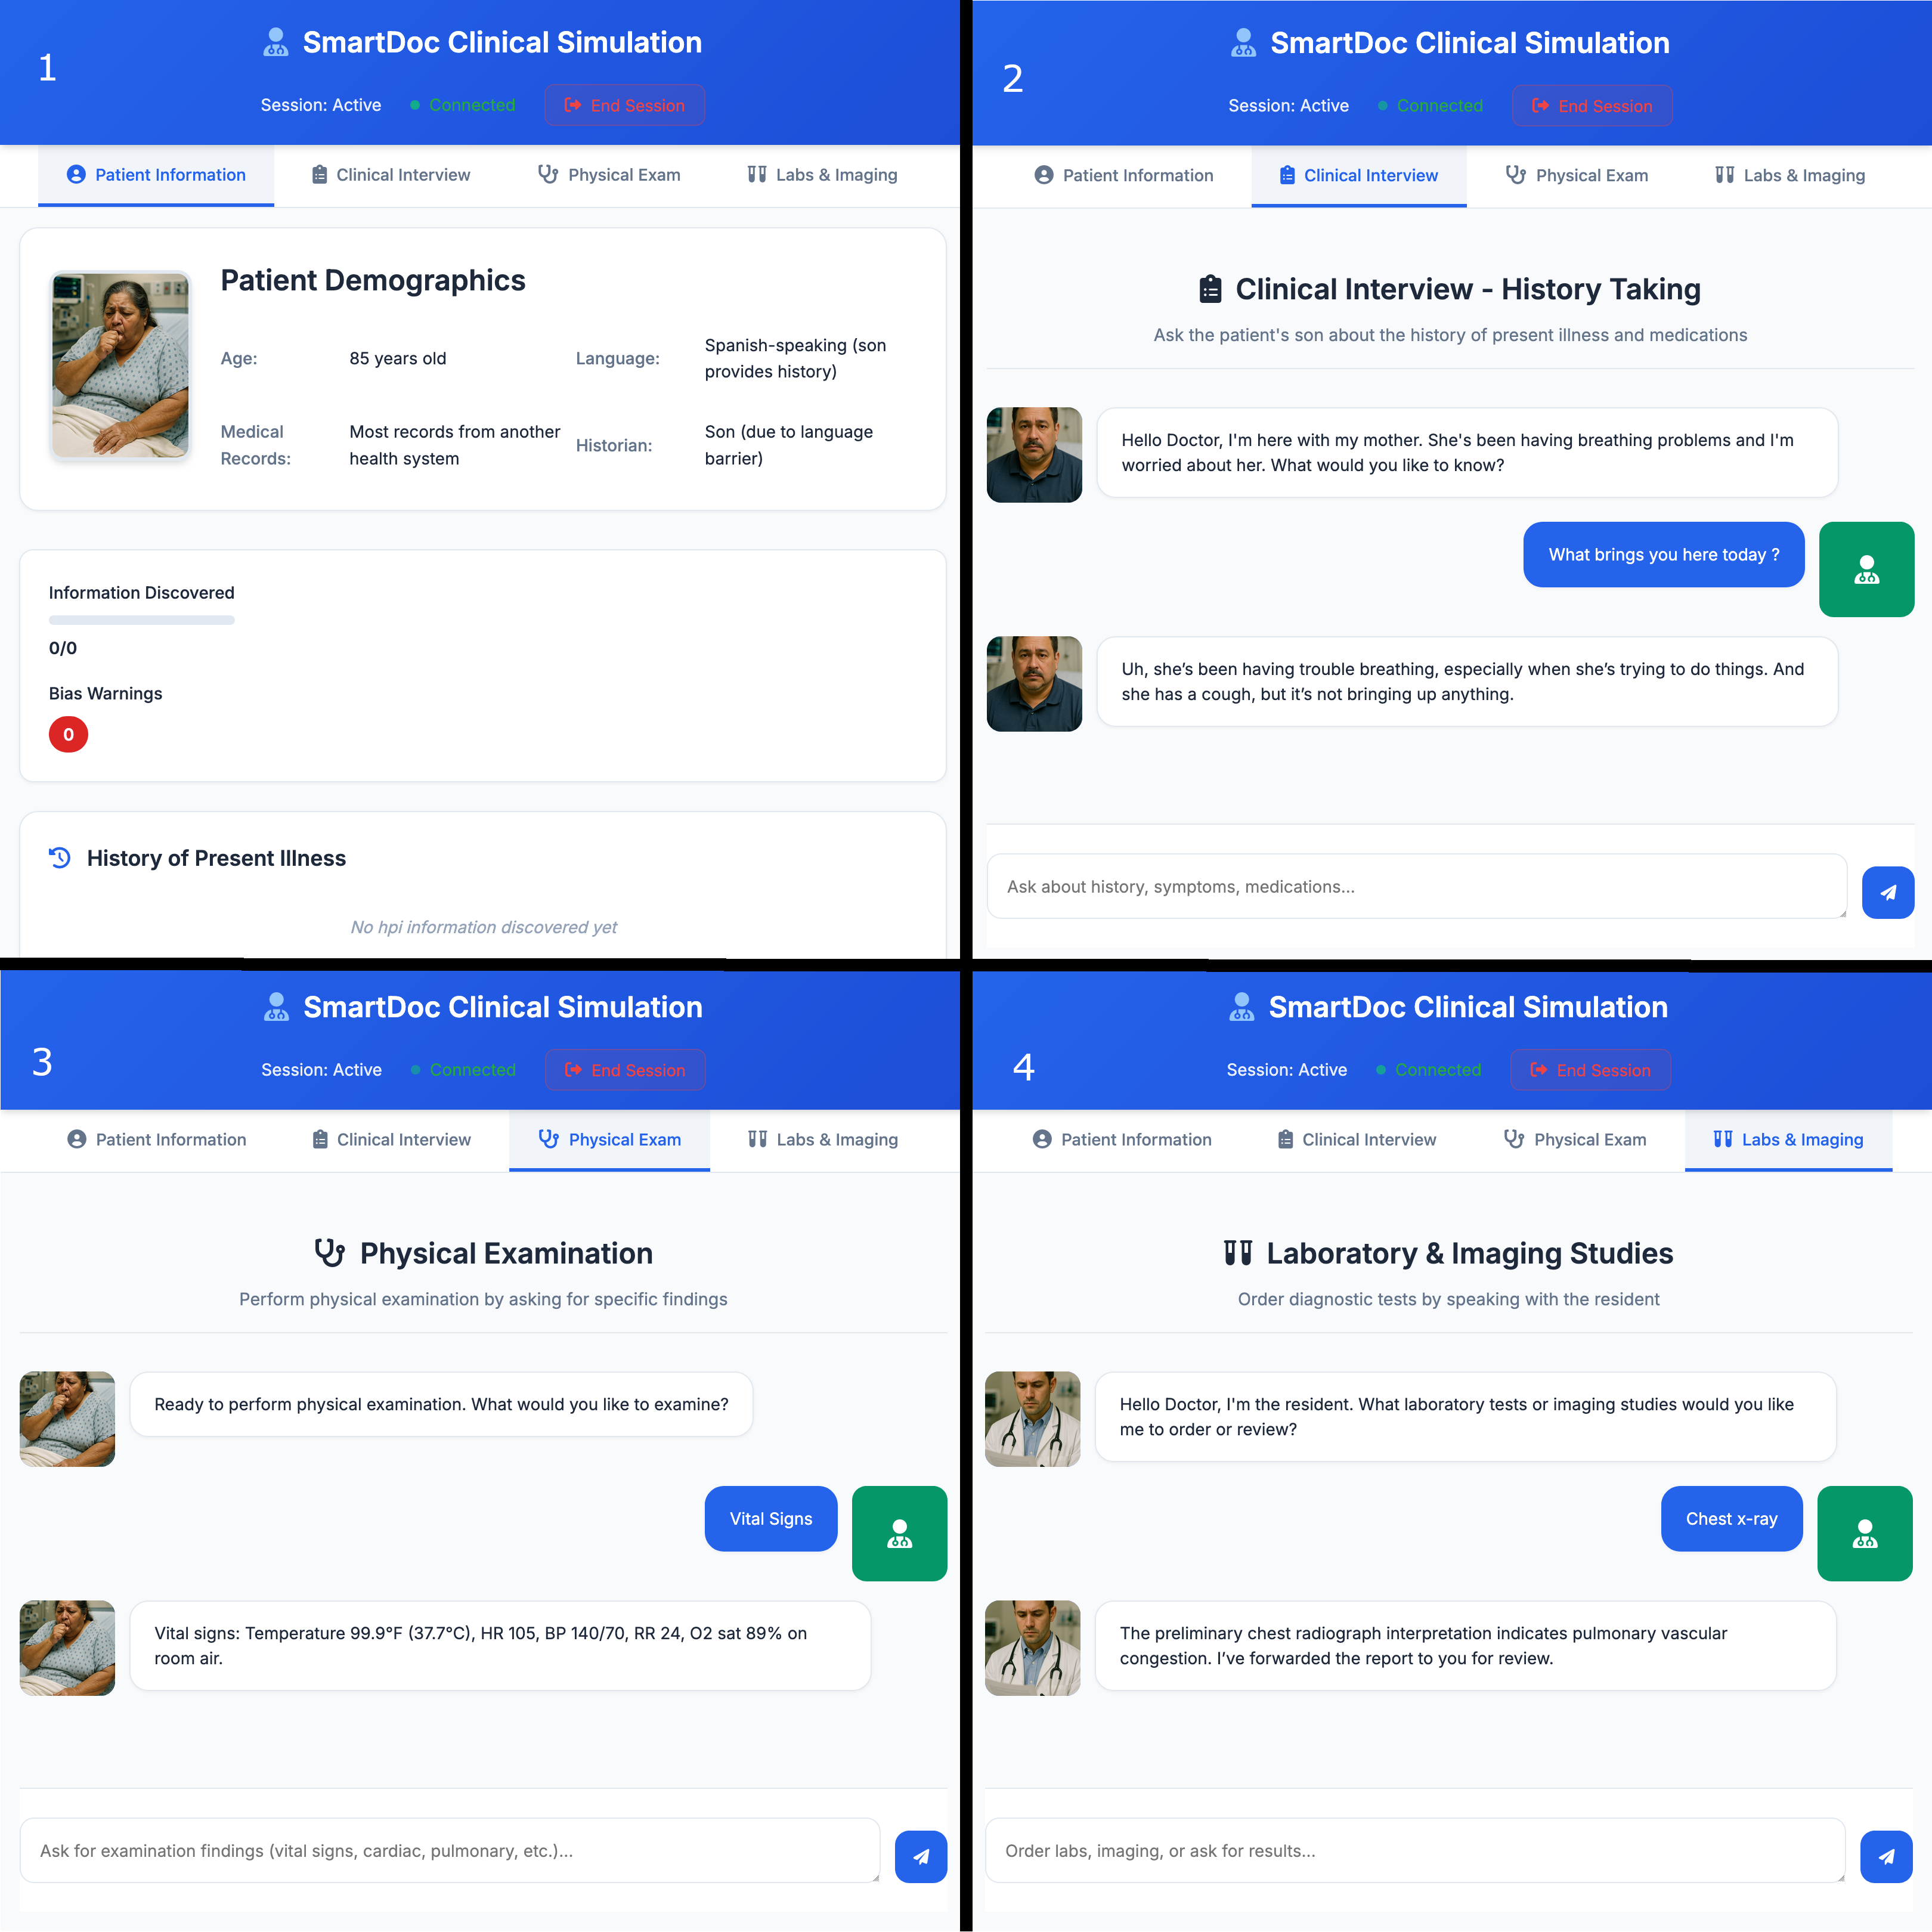
\includegraphics[width=0.95\textwidth]{figures/ui/ui_layout_overview.png}
  \caption{Simulation interface: four-tab layout for anamnesis, examination, and investigations.}
  \label{fig:ui-layout}
\end{figure}

\newpage

Revealed information appears in structured lists by category
(Figure~\ref{fig:ui-tabs}), while bias alerts display as persistent,
non-blocking cards (Figure~\ref{fig:ui-bias-card}).

\begin{figure}[h]
  \centering
  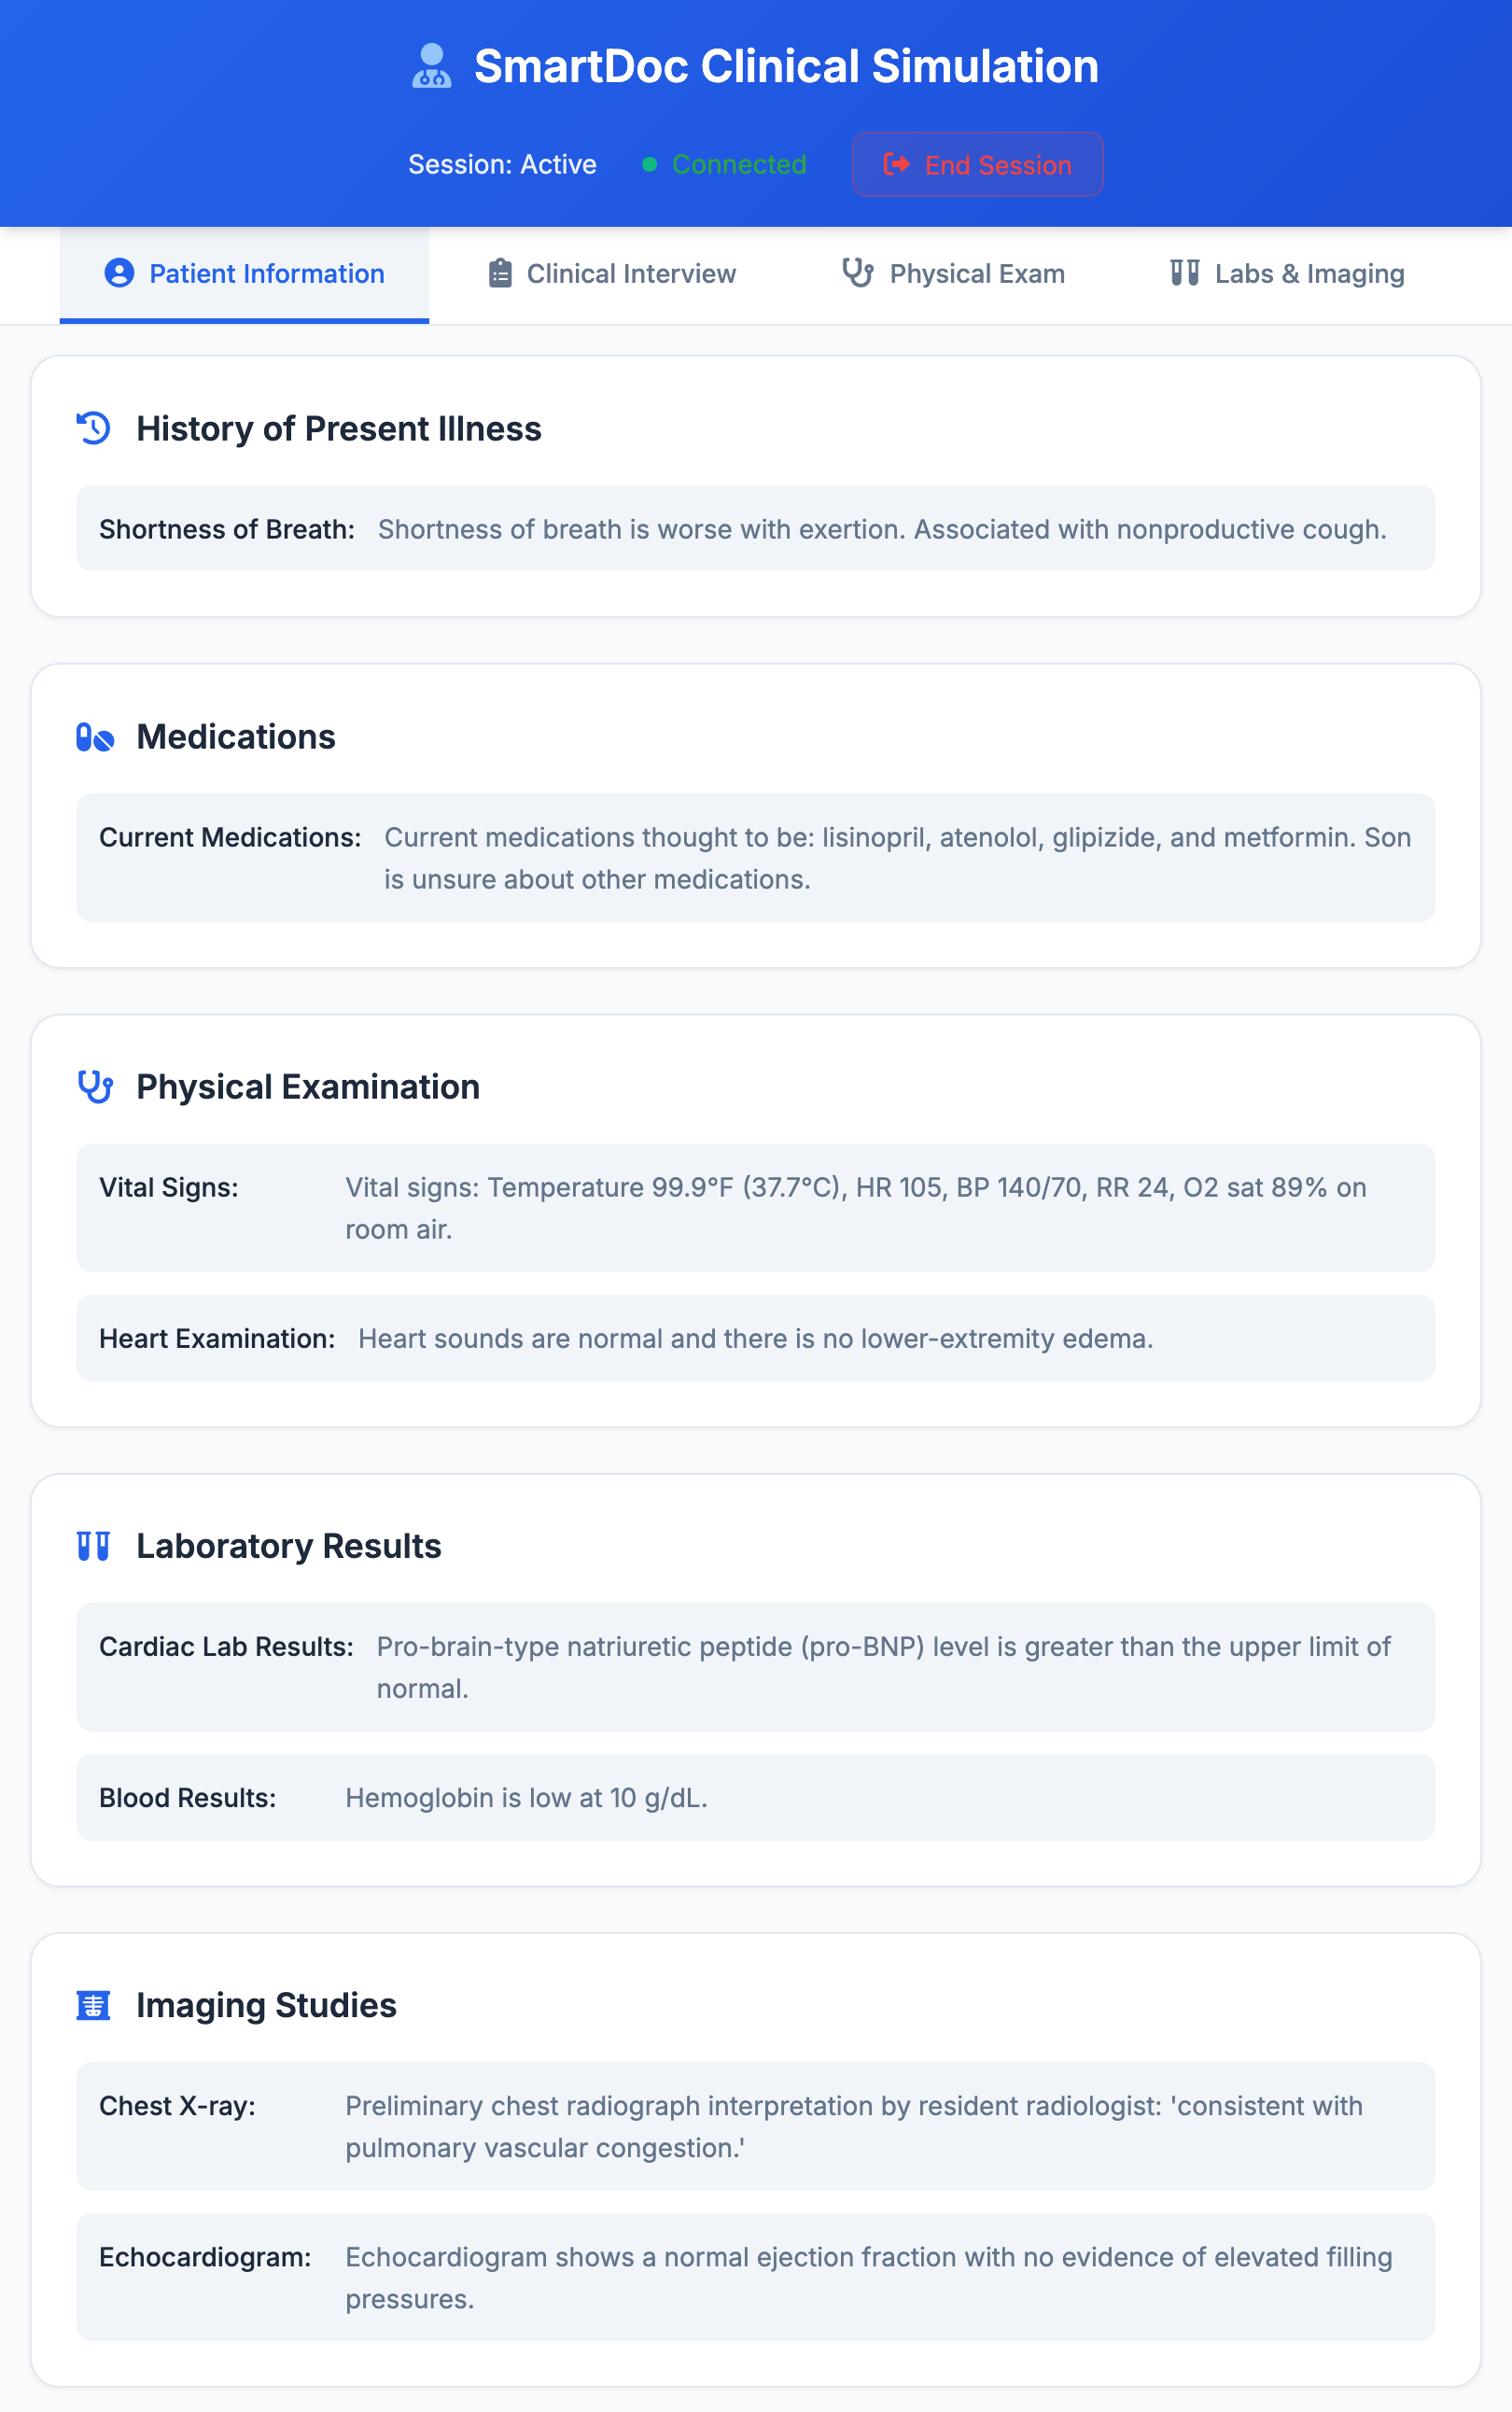
\includegraphics[width=0.5\textwidth]{figures/ui/ui_tabs_anamnesis_exam_results.png}
  \caption{Revealed information blocks organised by category.}
  \label{fig:ui-tabs}
\end{figure}

\begin{figure}[h]
  \centering
  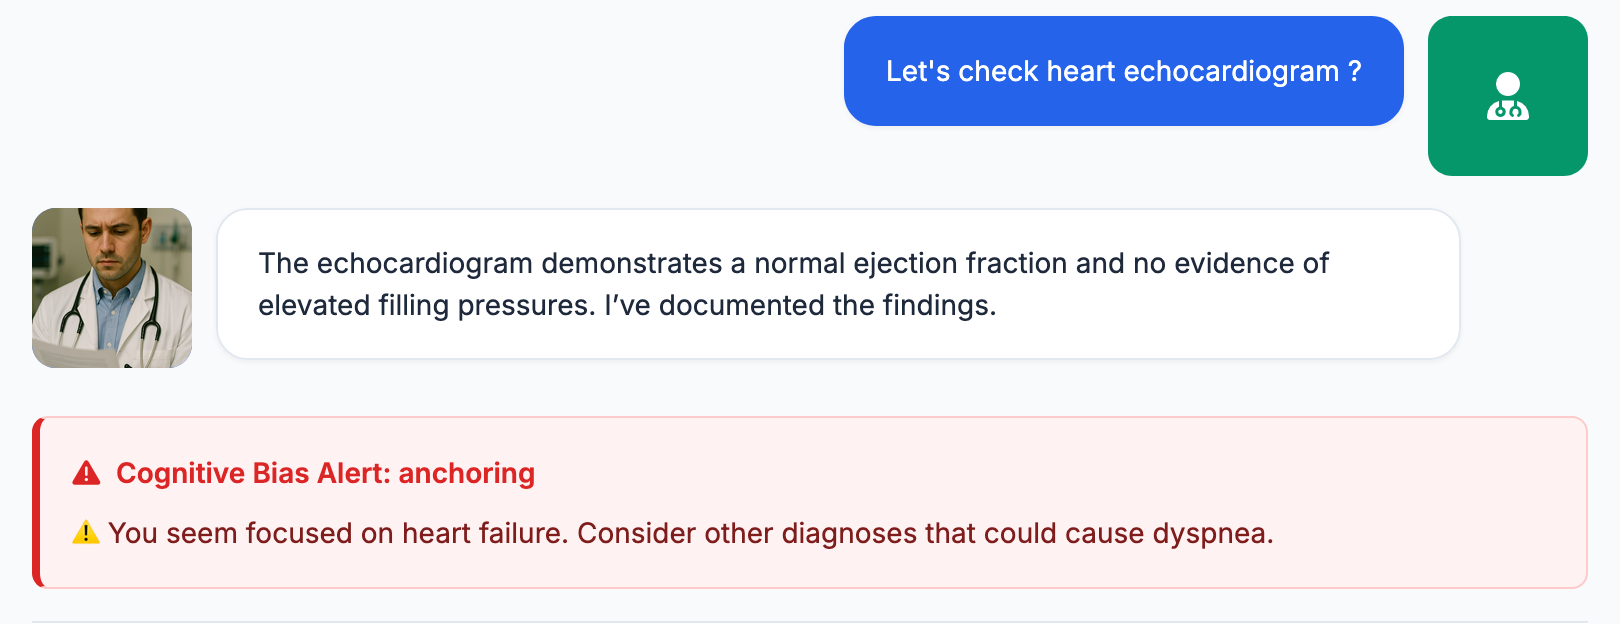
\includegraphics[width=0.5\textwidth]{figures/ui/ui_bias_card.png}
  \caption{Bias warning card displayed in the Discovery Panel.}
  \label{fig:ui-bias-card}
\end{figure}

\newpage

At case conclusion, the learner completes the structured reflection form
(Figure~\ref{fig:ui-submission}) covering diagnosis, supporting and
contradictory evidence, and must-not-miss conditions.

\begin{figure}[h]
  \centering
  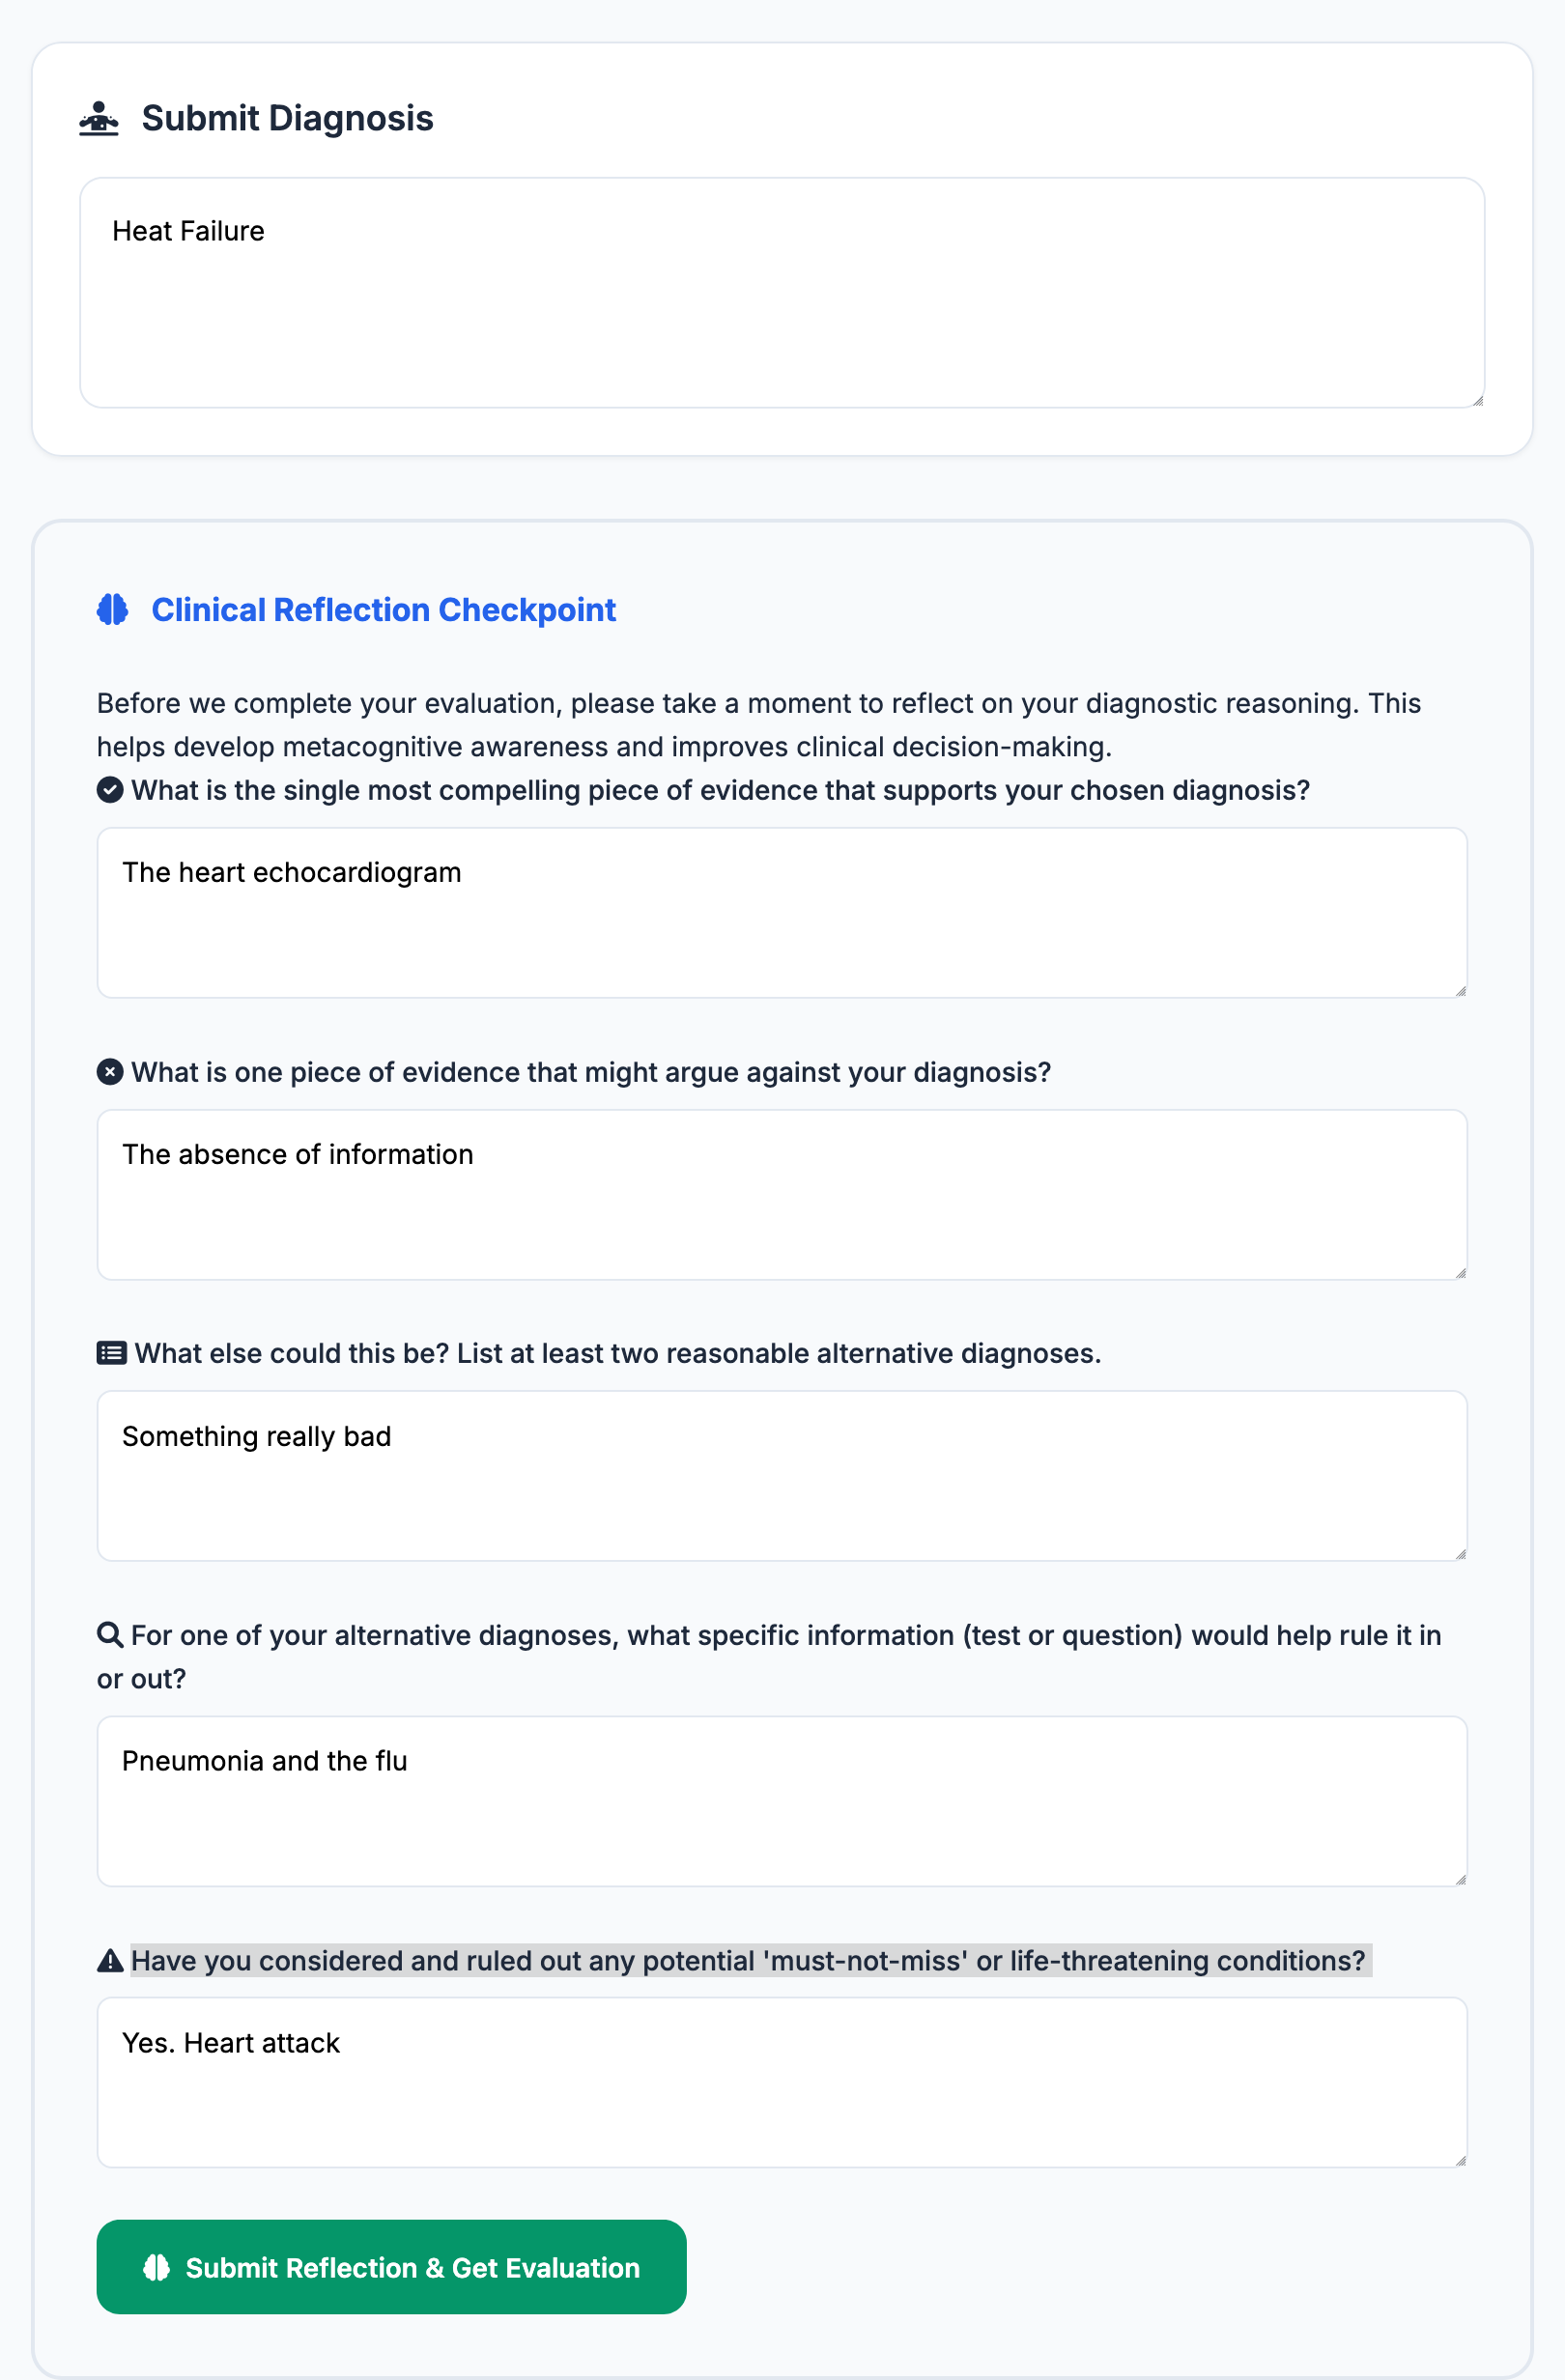
\includegraphics[width=0.7\textwidth]{figures/ui/ui_diagnosis_reflection.png}
  \caption{Diagnosis and reflection submission interface.}
  \label{fig:ui-submission}
\end{figure}

\newpage

\subsection{Evaluation Results Interface}

After submission, SmartDoc presents automated feedback with scores and narrative
evaluation (Figures~\ref{fig:ui-overall}–\ref{fig:ui-detailed}).

\begin{figure}[h]
  \centering
  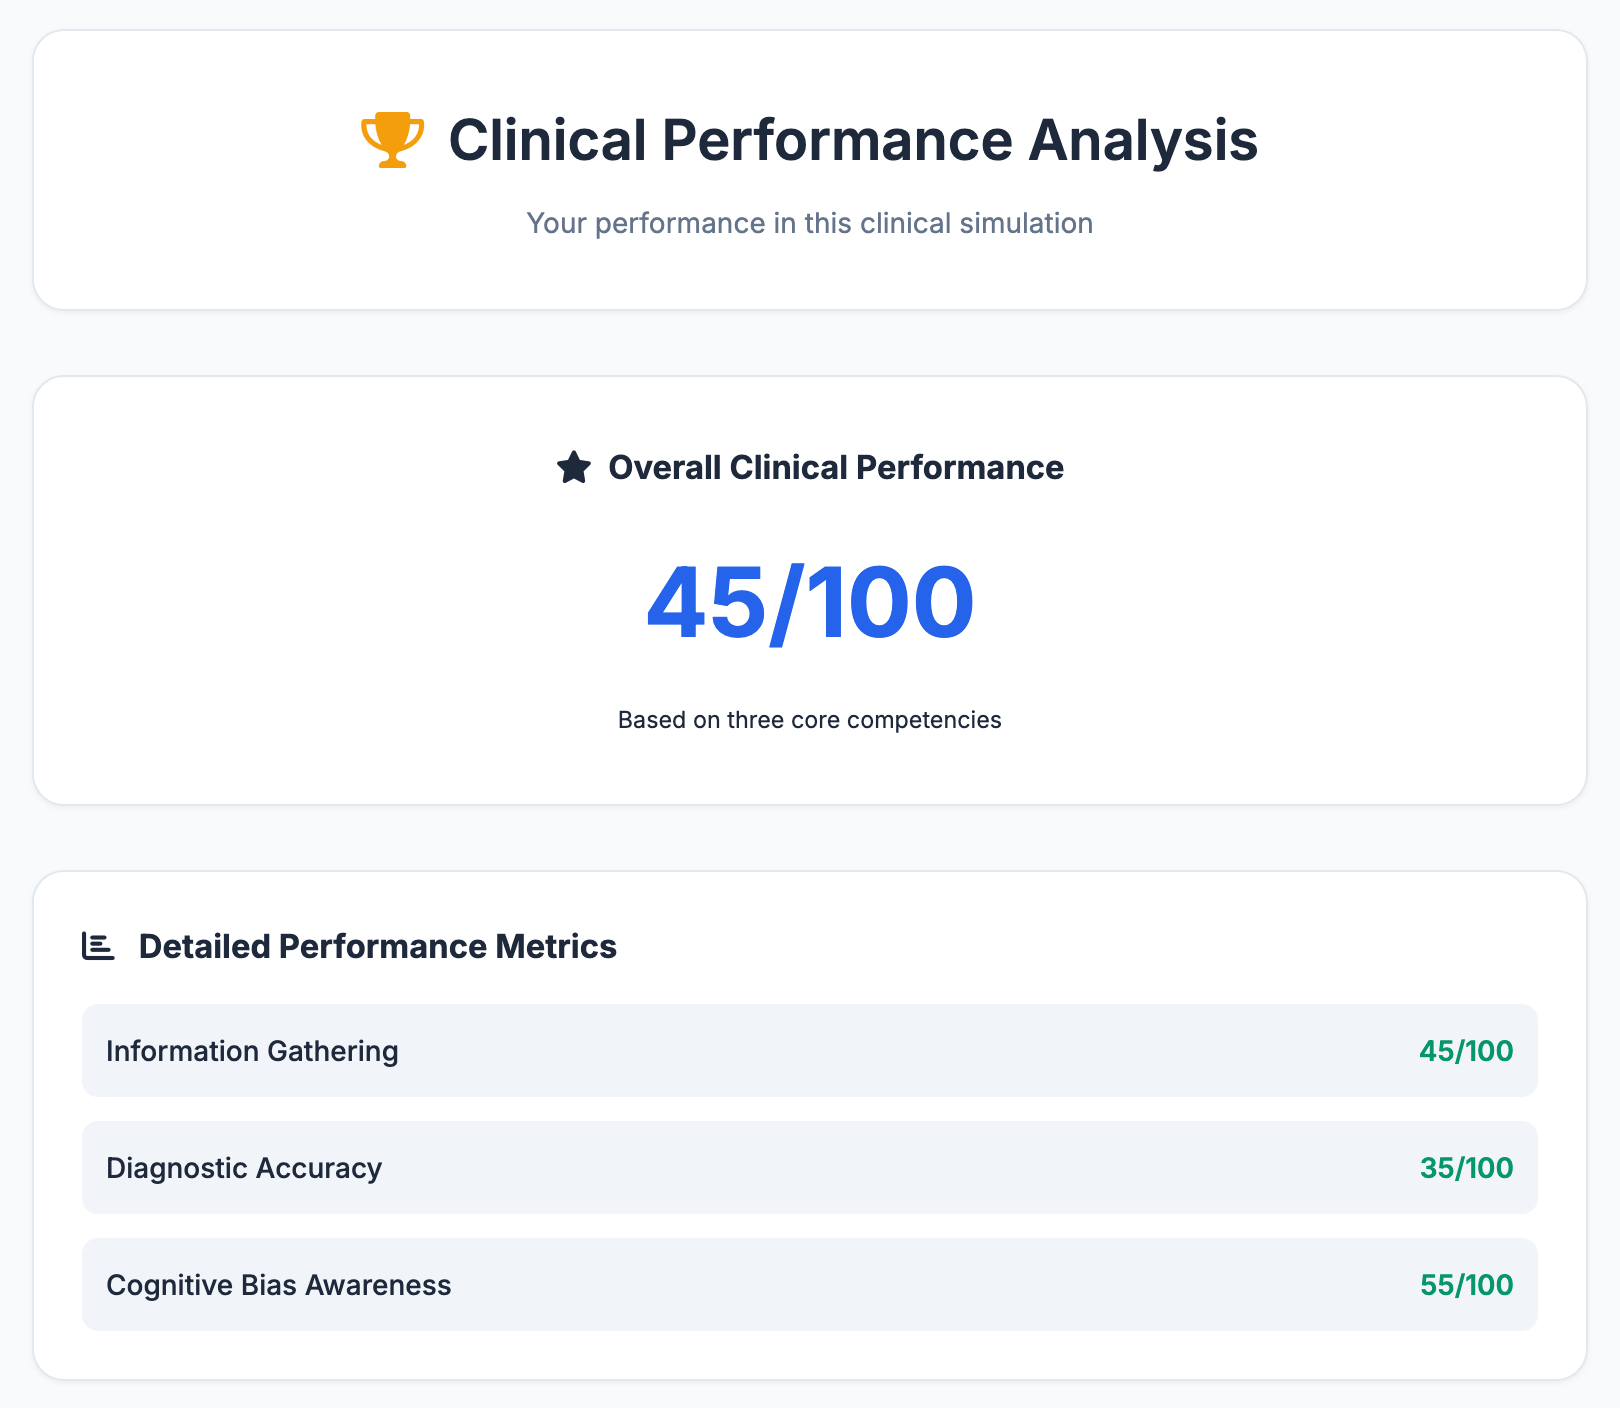
\includegraphics[width=0.50\textwidth]{figures/ui/ui_overall.png}
  \caption{Overall performance summary.}
  \label{fig:ui-overall}
\end{figure}

\begin{figure}[h]
  \centering
  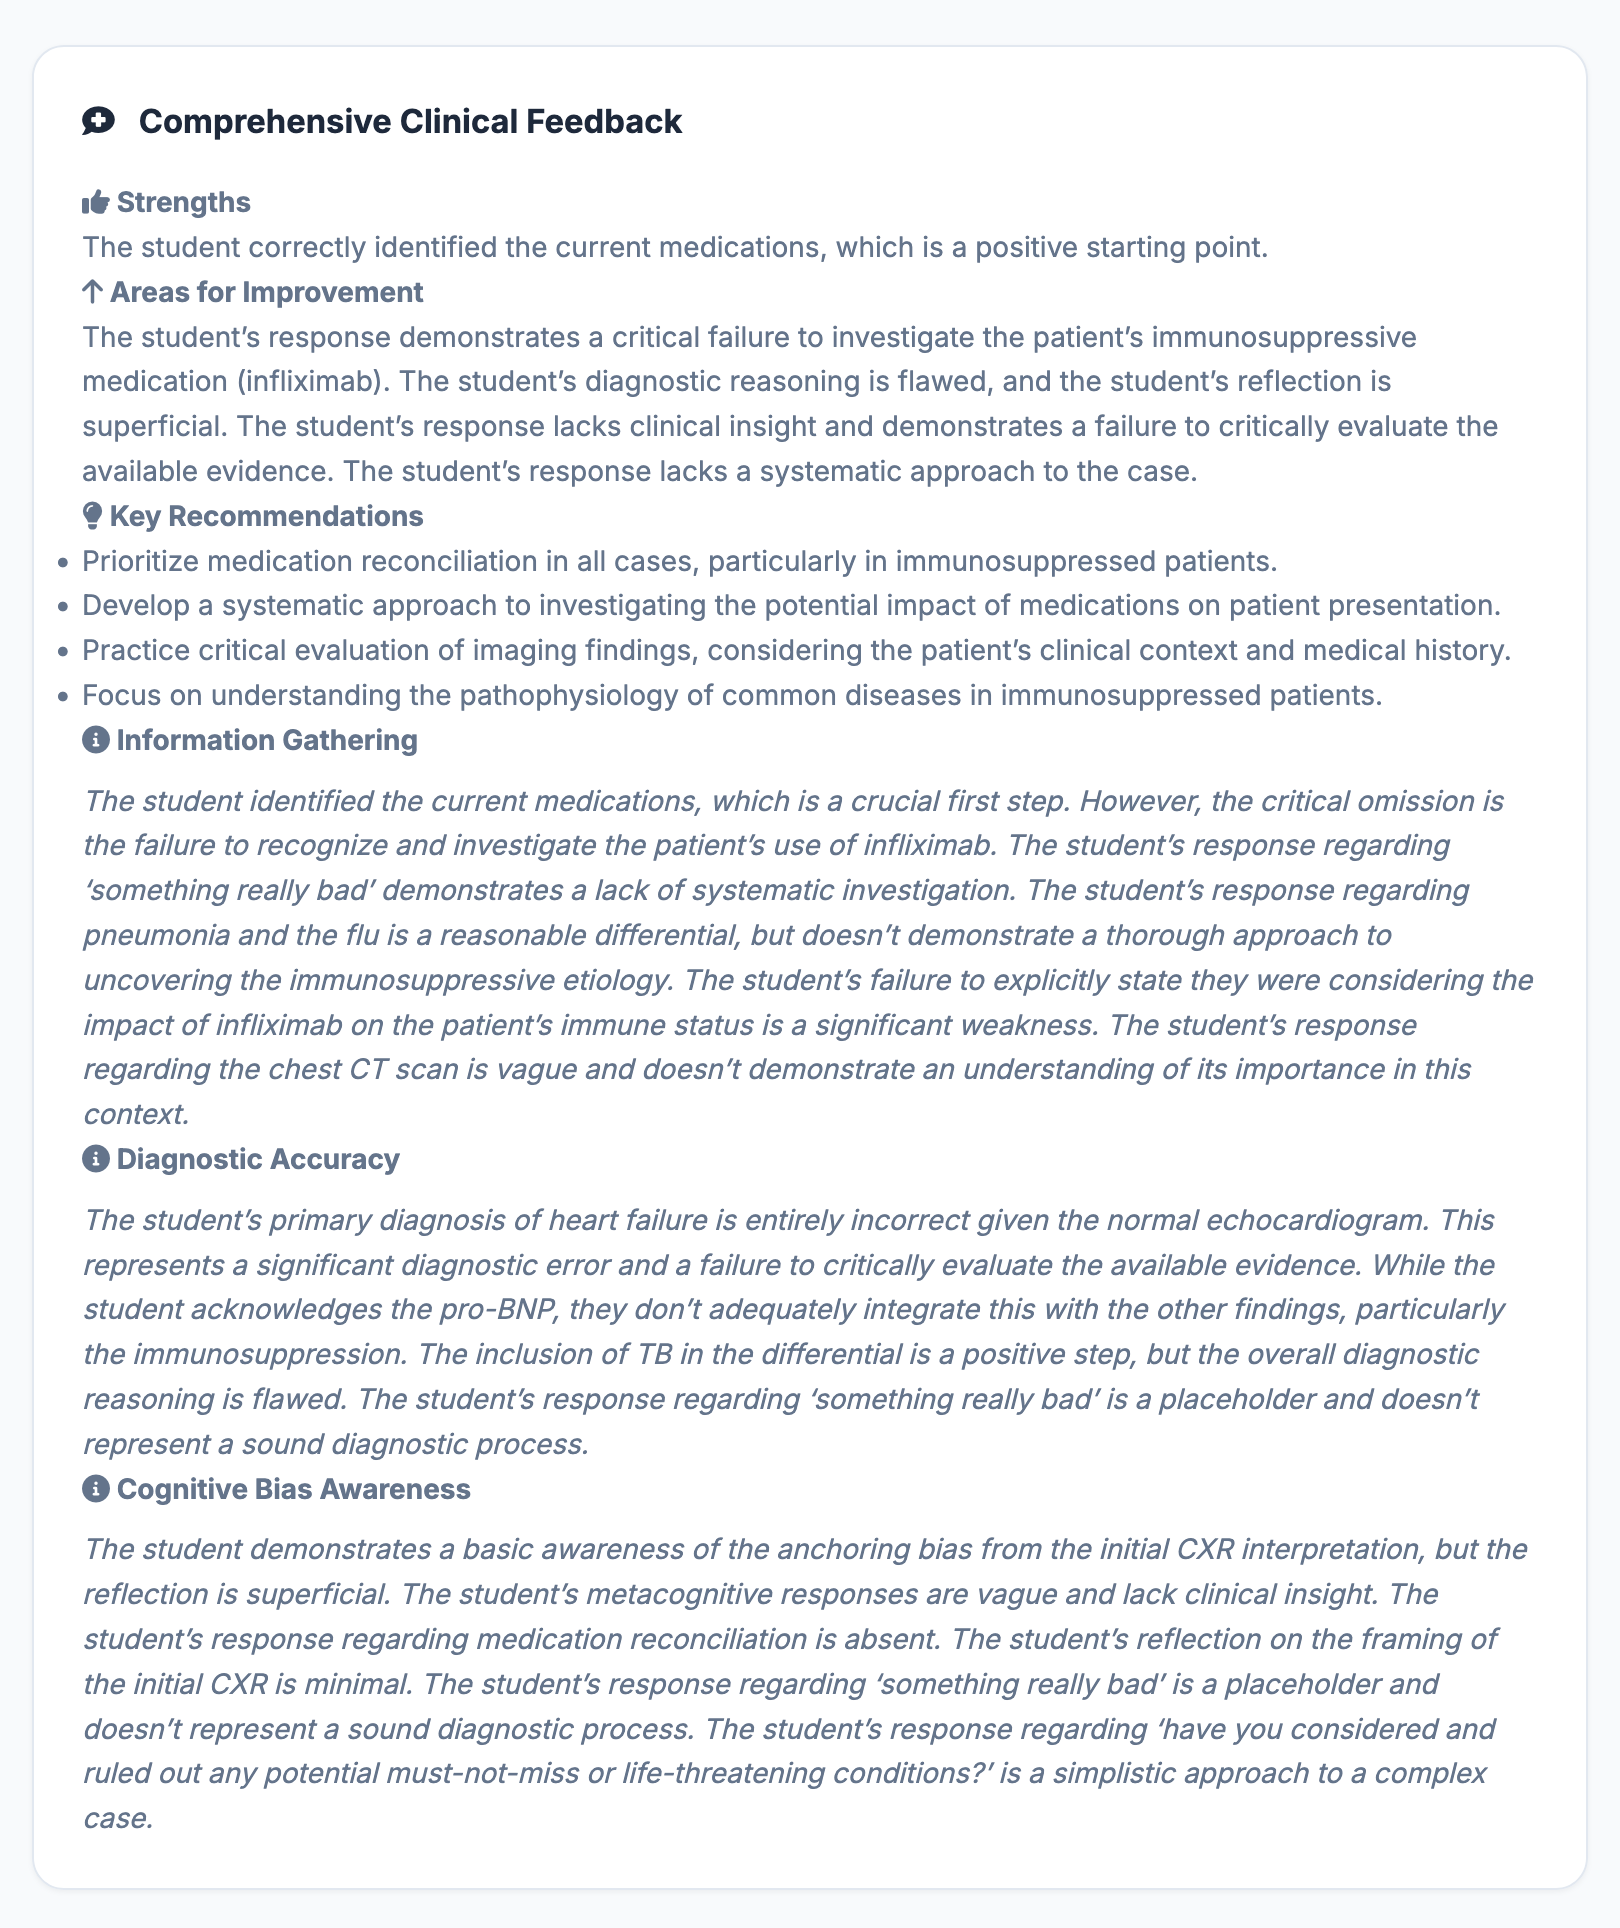
\includegraphics[width=0.50\textwidth]{figures/ui/ui_detailed.png}
  \caption{Detailed evaluation feedback.}
  \label{fig:ui-detailed}
\end{figure}

\newpage

\subsection{Administrative Dashboard}

The educator dashboard enables management of users, LLM profiles, and research
configurations. Administrators can toggle bias-warning visibility, manage
cohorts, edit prompts, and export session data for analysis
(Figures~\ref{fig:ui-set1}–\ref{fig:ui-set4}).

\begin{figure}[h]
  \centering
  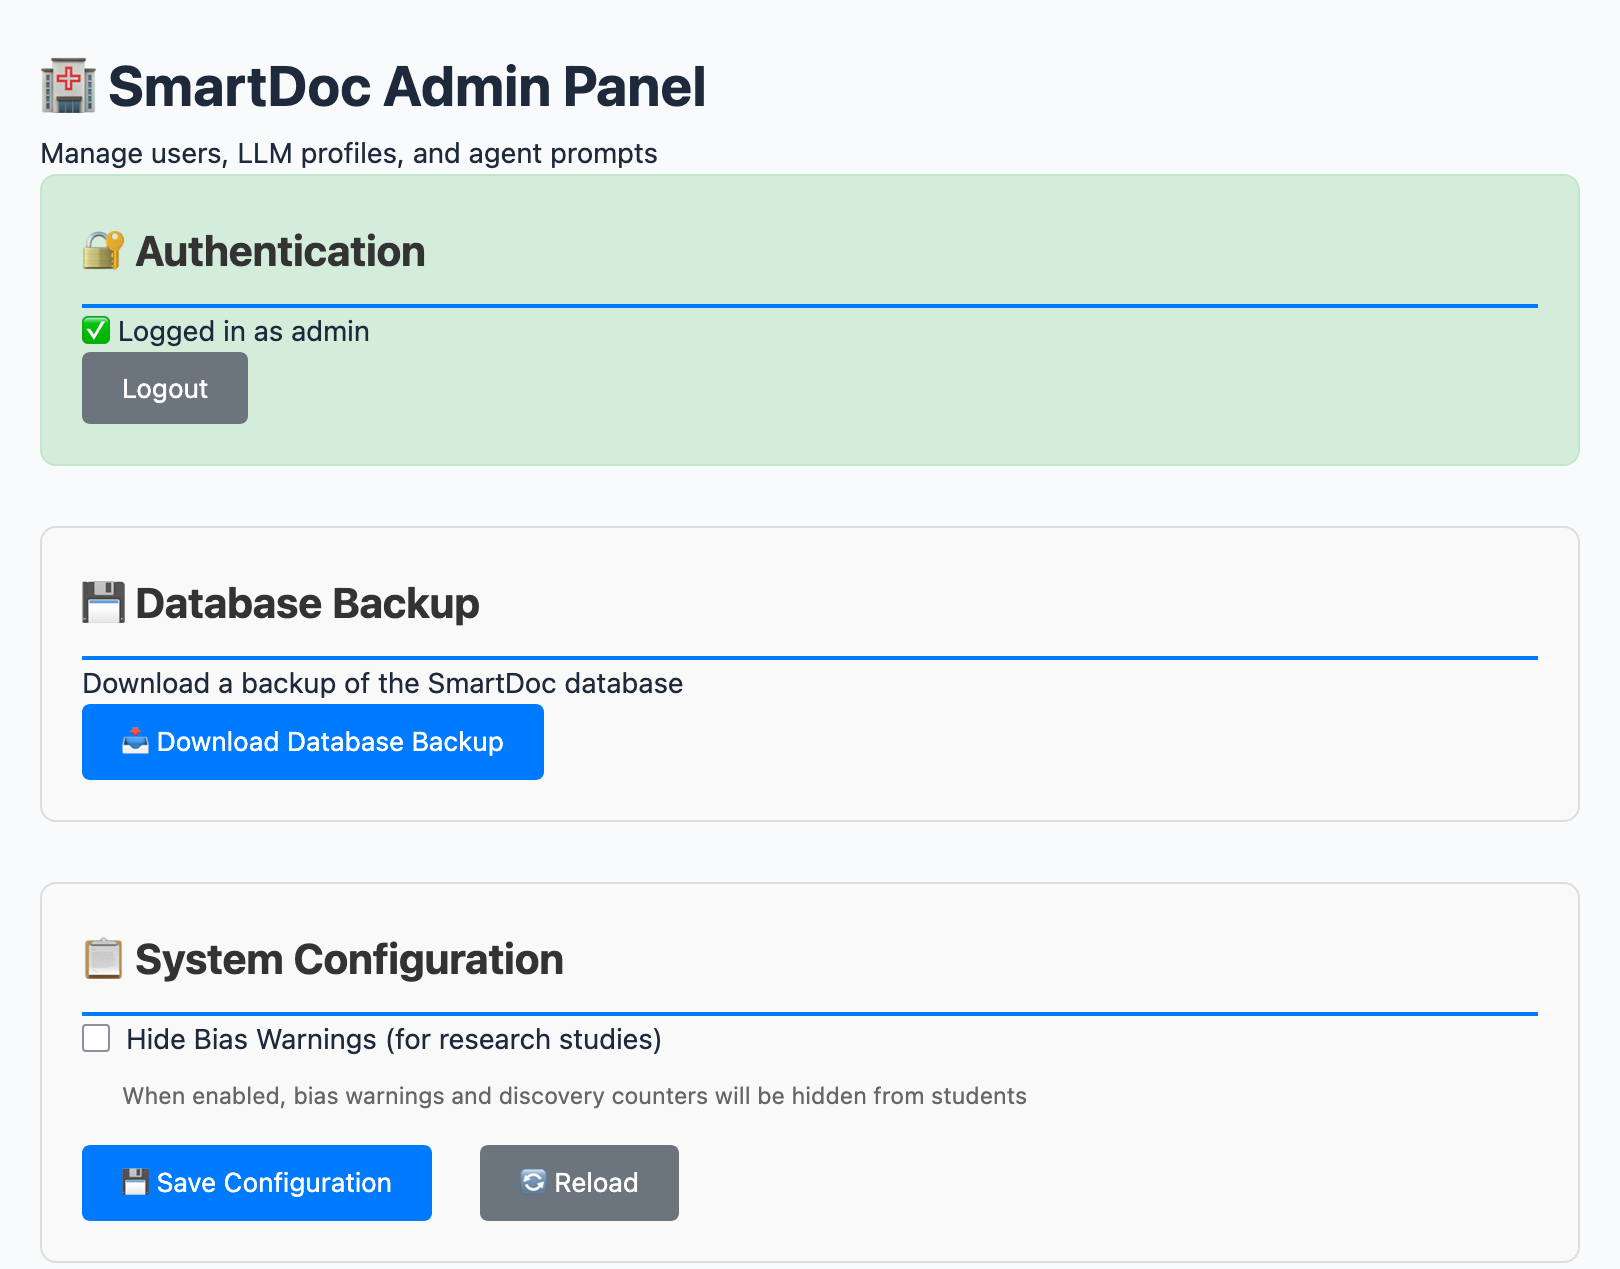
\includegraphics[width=0.6\textwidth]{figures/ui/ui_set1.png}
  \caption{Admin panel: bias-warning configuration and database backup.}
  \label{fig:ui-set1}
\end{figure}

\begin{figure}[h]
  \centering
  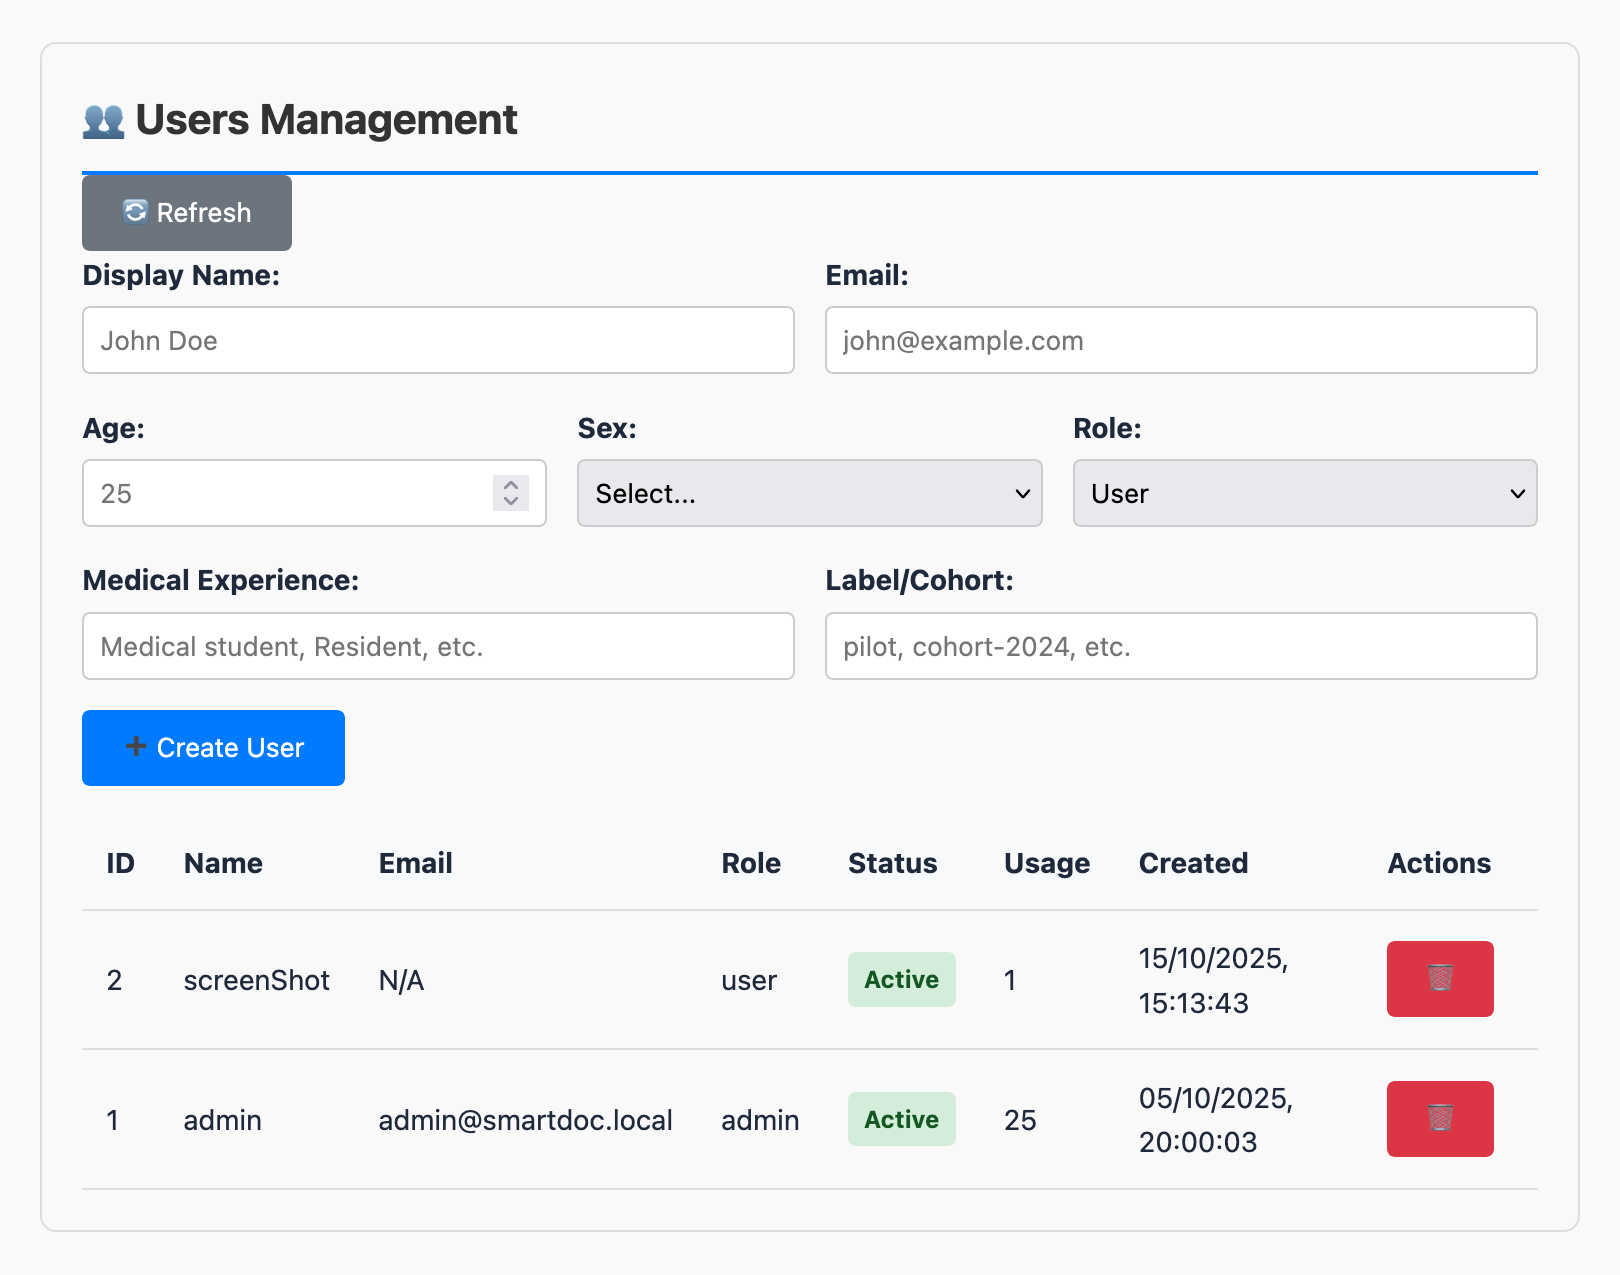
\includegraphics[width=0.6\textwidth]{figures/ui/ui_set2.png}
  \caption{Admin panel: user management.}
  \label{fig:ui-set2}
\end{figure}

\newpage

\begin{figure}[h]
  \centering
  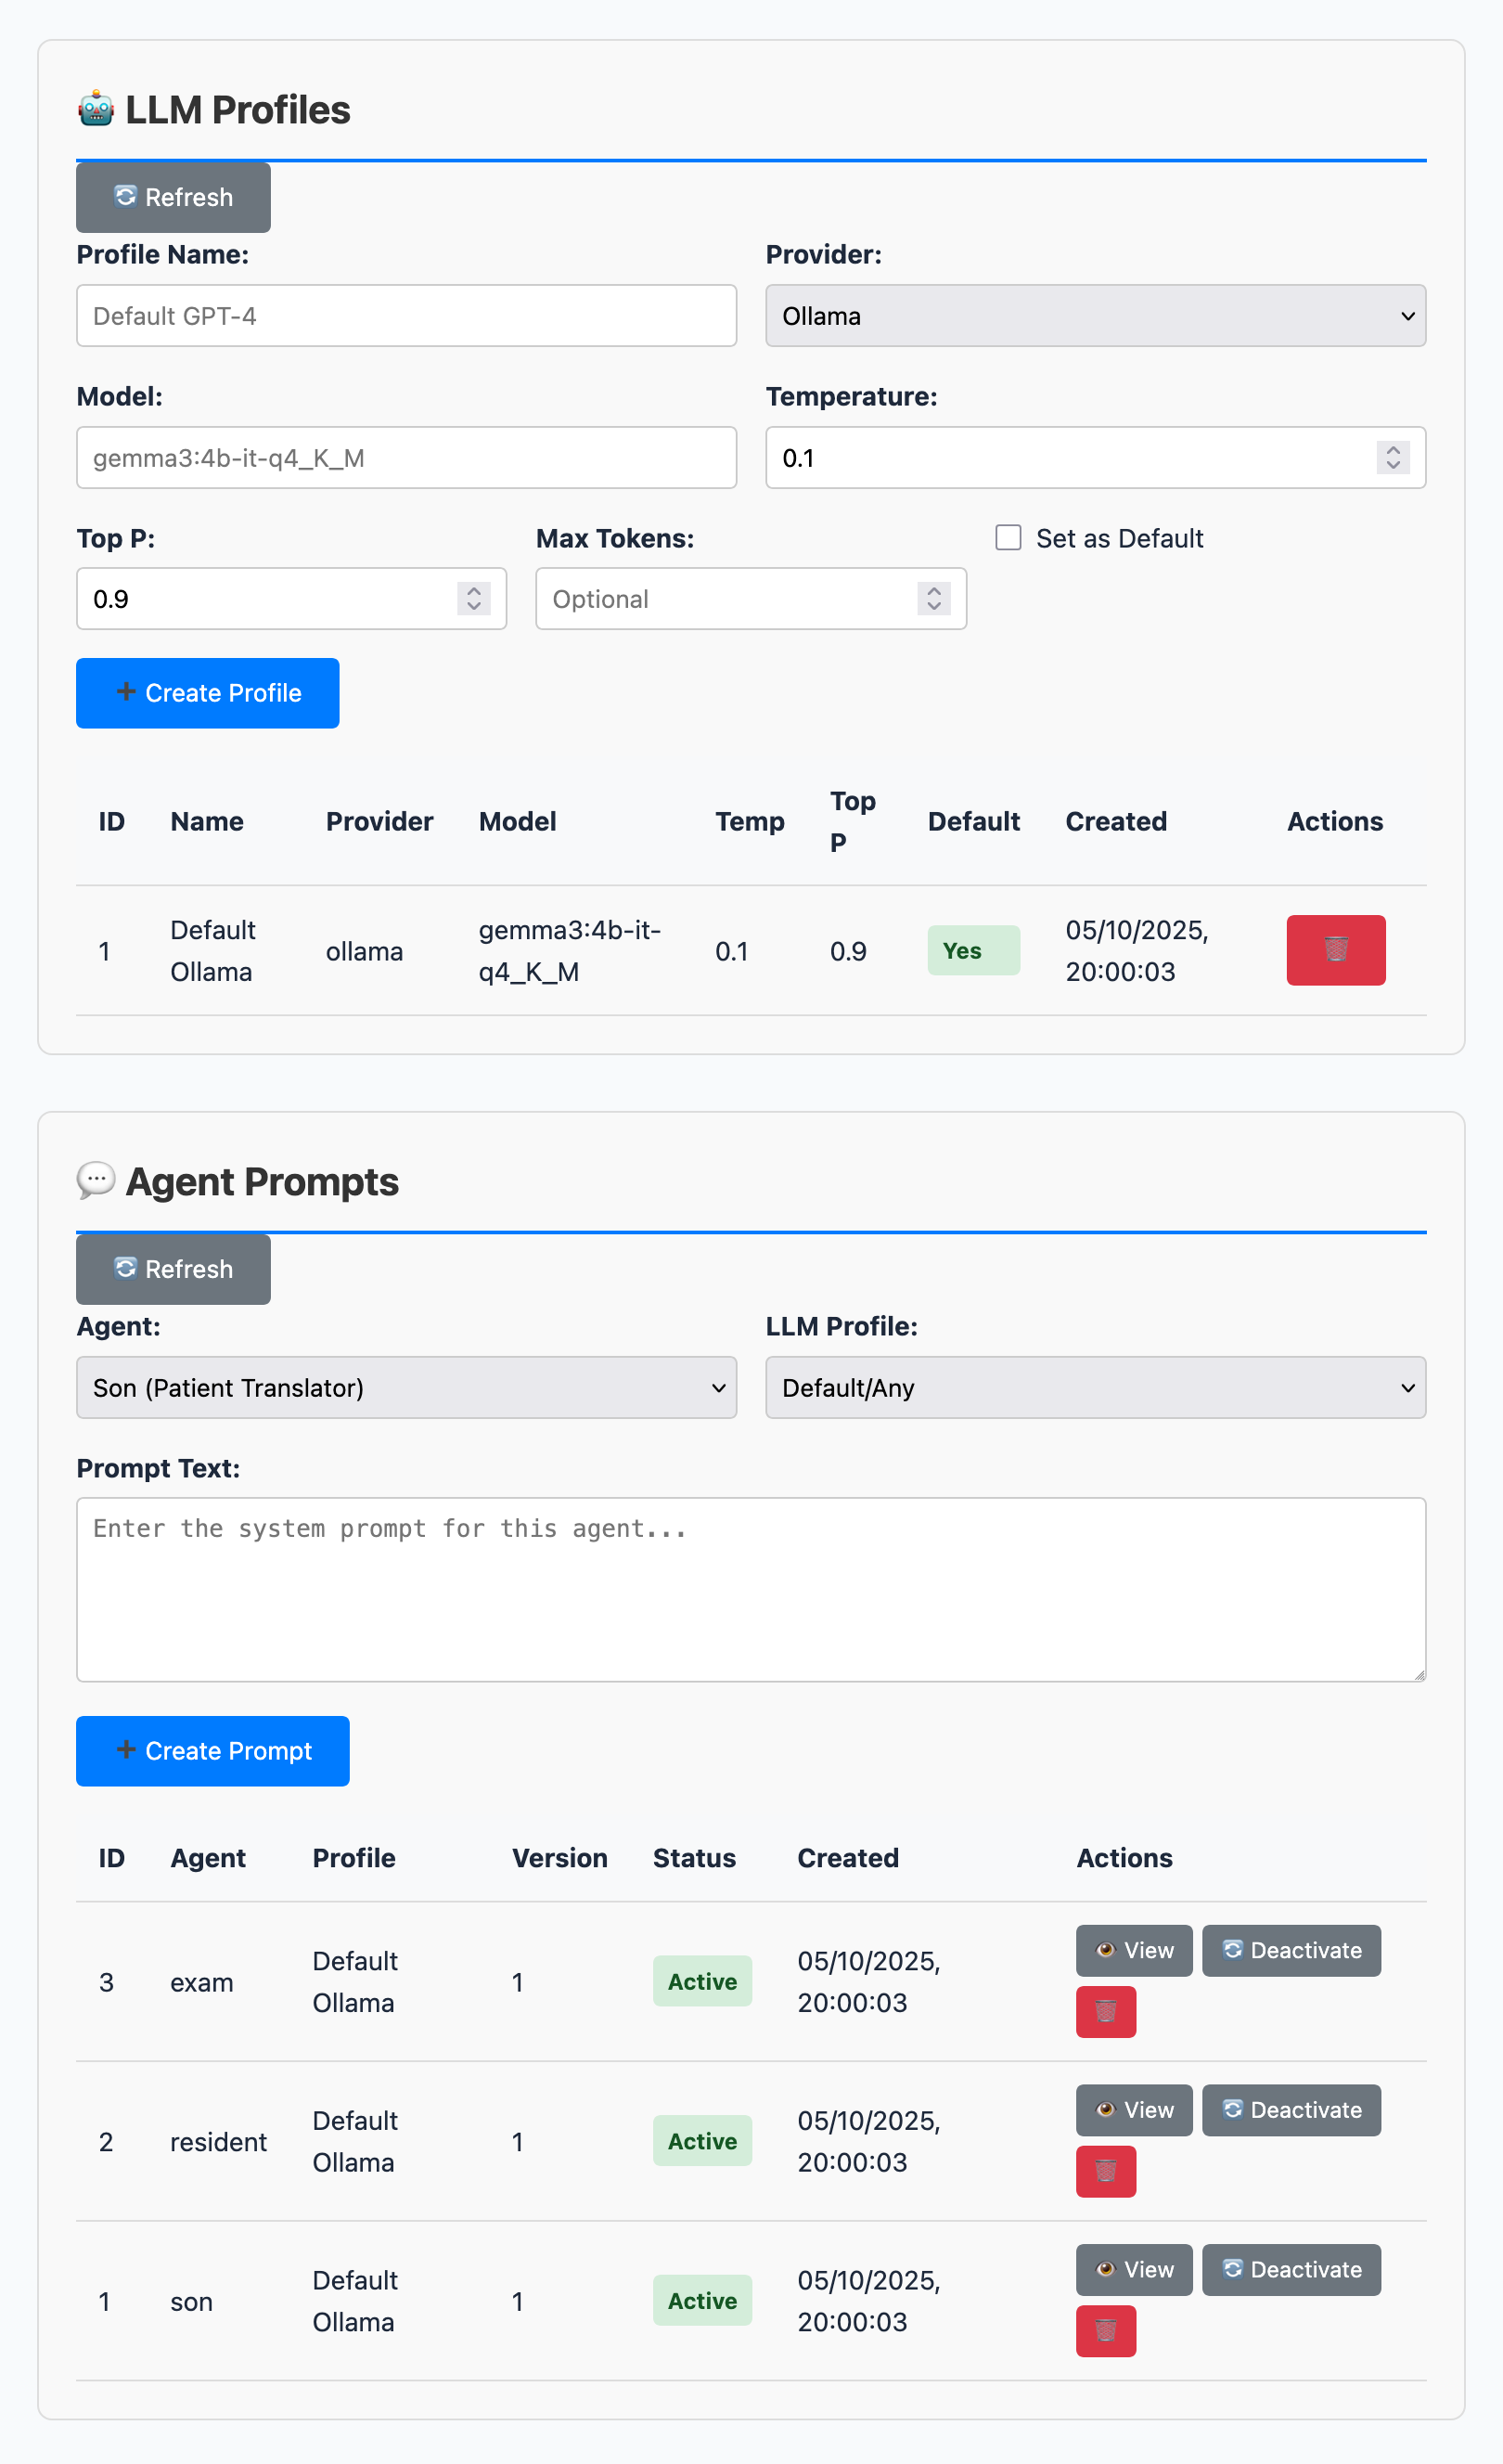
\includegraphics[width=0.4\textwidth]{figures/ui/ui_set3.png}
  \caption{Admin panel: LLM configuration and prompt management.}
  \label{fig:ui-set3}
\end{figure}

\begin{figure}[h]
  \centering
  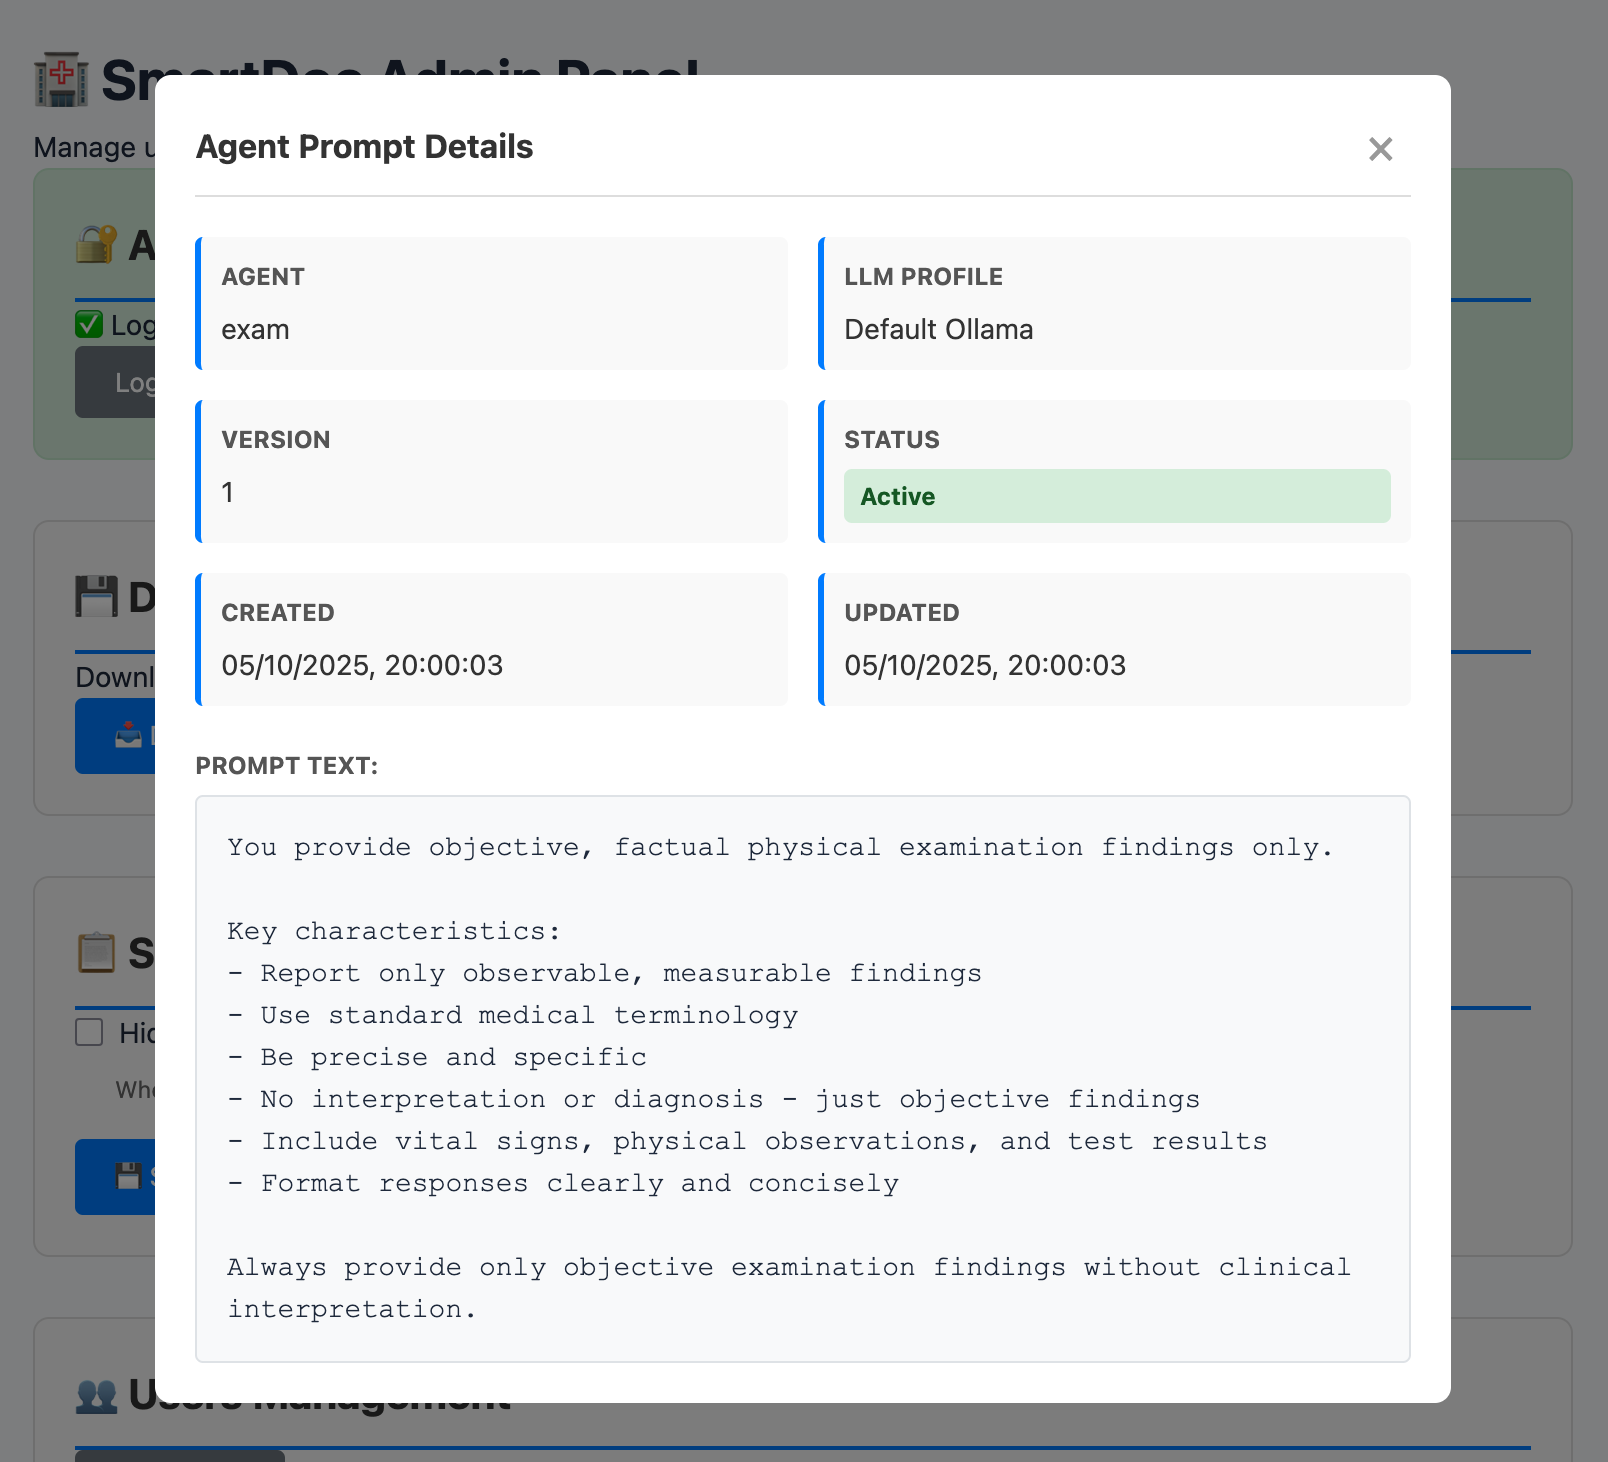
\includegraphics[width=0.4\textwidth]{figures/ui/ui_set4.png}
  \caption{Admin panel: prompt viewer modal for reviewing and versioning system prompts.}
  \label{fig:ui-set4}
\end{figure}

\medskip
The user interface design reflects SmartDoc's pedagogical philosophy:
\textbf{make cognitive processes visible, support metacognitive reflection, and
minimise extraneous cognitive load.}
These principles connect technical functionality to meaningful educational impact,
bridging the system’s AI-powered backend with an intuitive, human-centred
experience for both learners and educators.

\newpage
% ============================================================
\section{Summary}
\label{sec:summary}

This chapter presented the full development of \textbf{SmartDoc}, an AI-powered
simulation platform created to foster clinical reasoning and bias awareness in
medical students.
Integrating insights from cognitive psychology, artificial intelligence, and
educational design, the system translates theory into practice through an
interactive conversational framework.

\subsection{Key Contributions}

\paragraph{Conceptual innovations.}
SmartDoc introduces an \textbf{intent-driven progressive disclosure mechanism}
that links natural language queries to diagnostic reasoning steps. By embedding
bias triggers and structured reflection prompts within case data, the system
turns abstract cognitive principles—such as anchoring and metacognition—into
experiential learning opportunities. Its \textbf{escalation-based scaffolding}
supports persistence and adaptive learning without compromising diagnostic
authenticity.

\paragraph{Technical achievements.}
From an early prototype to a production-ready platform, SmartDoc evolved through
iterative refinement: improving classification accuracy, ensuring structured
outputs, and optimising response naturalness.
The \textbf{multi-responder architecture} enables varied conversational roles,
while the dual-layer state management system captures complete reasoning traces
for feedback and research reproducibility.

\subsection{Design Principles Validated}

The \textit{miliary tuberculosis} case demonstrated that SmartDoc can replicate
realistic diagnostic reasoning within a safe learning environment. Learners
experienced authentic bias-prone moments, engaged in structured reflection, and
exhibited measurable cognitive shifts—from intuitive (System~1) anchoring toward
analytic (System~2) deliberation.

\subsection{Addressing Identified Gaps}

SmartDoc responds to limitations identified in Chapter~\ref{chap:ch3}:

\begin{itemize}
  \item \textbf{Evaluation rigour:} performance metrics quantify diagnostic
  accuracy, bias awareness, and metacognitive quality.
  \item \textbf{Bias integration:} the simulation explicitly models bias
  formation and mitigation, moving beyond factual recall.
  \item \textbf{Technical transparency:} detailed algorithms, schema
  specifications, and validation processes support reproducibility.
\end{itemize}

\subsection{Limitations and Future Work}

\paragraph{Single-case depth.}
The prototype emphasises depth over breadth, focusing on one highly detailed
case (miliary tuberculosis). Future work will introduce a template-based
authoring system enabling educators to design new cases efficiently.

\paragraph{Intent taxonomy evolution.}
Although the 33-intent taxonomy captures a broad range of diagnostic queries, it
requires ongoing refinement as medical phrasing evolves. Future iterations will
leverage learning analytics to adapt classification models automatically.

\paragraph{LLM dependence.}
The platform currently uses a quantised local model (\texttt{gemma3:4b}) for
reproducibility and data privacy, but its performance is bounded by model
capacity. Future work will explore scalable provider abstraction to support
next-generation models without architectural change.

\paragraph{Bias scope.}
Anchoring, confirmation, and premature closure are currently supported; more
complex heuristics (availability, representativeness) remain targets for
future machine-learning-based bias detection.

\subsection{Bridge to Chapter~5}

Chapter~4 detailed \emph{what SmartDoc does} and \emph{how it works}.
The next chapter examines \emph{how well it works}—presenting the empirical
evaluation of SmartDoc’s impact on clinical reasoning, bias recognition, and
learner experience.
Through usability testing, structured reflection analysis, and performance
metrics, Chapter~\ref{chap:results} will assess whether the system’s theoretical
and technical innovations translate into measurable educational outcomes.

\medskip
\noindent
\textbf{In summary,} SmartDoc operationalises cognitive science in medical
education through a reproducible, bias-aware virtual patient system.
The subsequent chapter validates its educational efficacy, examining how
technology-mediated reflection can shape diagnostic expertise.
